\documentclass{hsflensburg}
\title{Bewegungserkennung auf mobilen Geräten mit Verwendung von GANs für eine
automatische Datensatzgenerierung}
\subtitle{Master-Thesis}

\author{
  \name{Florian Hansen}\\
  \institution{Hochschule Flensburg}
}

\usepackage[ngerman]{babel}
\usepackage{csquotes}
\usepackage{biblatex}
\usepackage{amsmath}
\usepackage{amssymb}
\usepackage{mathtools}
\usepackage{tabularx}
\usepackage{amssymb}
\usepackage[locale=DE]{siunitx}
\usepackage[ngerman,linesnumbered,algoruled,boxed,lined]{algorithm2e}
\addbibresource{bibliography.bib}

\sisetup{
  group-digits=true,
  group-separator=\, ,
  group-minimum-digits=5,
  detect-all
}

\newtheorem{definition}{Definition}

\setcapindent{0pt}

\begin{document}
  \maketitle
  \newpage \ \newpage
  \tableofcontents
  \newpage \ \newpage

  \chapter{Einleitung}
Kann eine Bewegungserkennung mithilfe von künstlichen neuronalen Netzen
effizient und in Echtzeit auf mobilen Geräten wie Smartphones ausgeführt
werden? Mit dieser Frage beschäftigt sich diese Arbeit. Speziell wird
sich dabei auf die Erkennung von Bewegungen bezogen. Dabei soll untersucht
werden, wie Machine-Learing-Modelle auf mobile Geräte übertragen werden können,
um eine Echtzeiterkennung durchführen zu können. Künstliche Intelligenz hat
bereits in vielen verschiedenen Bereichen eine unterstützende Rolle
eingenommen.  Dementsprechend ist das Feld in den letzten Jahren stetig
gewachsen und hat an Interesse gewonnen. Viele Anwendungen funktionieren nur
deshalb, weil sie durch Modelle des Machine-Learnings unterstützt werden. Vor
allem in der Computer-Vision findet diese Technologie Anwendung. Beispiele
hierfür sind Bildklassifizierer und Objekt-Detektoren, die entsprechend Bilder
einer Klasse zuordnen bzw. viele Objekte innerhalb eines Bildes erkennen. Neben
der Bildverarbeitung ist die Erkennung von menschlichen Posen bzw. von
Bewegungen mit künstlichen neuronalen Netzen (KNN) ein weiteres, aktuelles
Forschungsthema. Diese Art von Detektoren werden unter anderem dazu verwendet,
um Schlüs\-sel\-punkte des menschlichen Körpers zu identifizieren.

Während solche Modelle bereits im Desktopbereich mit weniger Einschränkungen
ausgeführt werden können, sind diese eher schwierig auf ressourcenarme Geräte
übertragbar. Oft müssen abgewandelte, verkürzte Varianten erstellt werden, um
die benötigte Rechenleistung so gering wie möglich zu halten -- die meisten
Smartphones haben zur Zeit leider nicht die gleichen Rechen- und
Speicherkapazitäten wie die meisten Desktopmaschinen, ganz zu schweigen von
diversen anderen Geräten des Internet-of-Things (IoT) wie Haushaltsgeräte und
Sensoren. Aus diesem Grund soll sich diese Arbeit insbesondere damit
beschäftigen, wie die Bewegungserkennung auf mobilen Geräten ausgeführt werden
kann. Zusätzlich wird untersucht, welche Anpassungen vorhandene
Machine-Learning-Modelle benötigen, um auf mobilen Geräte ausgeführt werden zu
können.

Kapitel \ref{chapter:basics} beschäftigt sich mit den Grundlagen der in dieser
Arbeit verwendeten Technologien. Dabei wird unter anderem darauf eingegangen,
wie Unterschiede zwischen Distributionen gemessen werden können, um damit den
Grundstein für spätere Loss-Funktionen zu schaffen. Diese werden dann vor allem
für das Trainieren von Generative-Adversarial-Networks (GANs) verwendet. Auch
werden in diesem Kapitel einige Grundbausteine zum Entwickeln von sehr tiefen
neuronalen Netzen besprochen. Anschließend wird die Funktionsweise von GANs und
entsprechenden Verlustfunktionen zum Trainieren dieser Netzwerke thematisiert.
Des Weiteren werden Probleme der einzelnen Architekturen aufgezeigt und Lösungen
vorgestellt.

Kapitel \ref{chapter:dataset} stellt Methoden vor, die zum Erstellen eines
Datensatzes verwendet werden. Dieser Datensatz wird anschließend verwendet, um
die Bewegungserkennung aus dem nächsten Kapitel zu implementieren und die
Modelle damit zu trainieren. Besonders wird in diesem Kapitel der Aufbau des
Datensatzes erläutert und inwiefern dieser mithilfe von GANs erweitert werden
kann. Insbesondere wird hier versucht, einen kompletten Datensatz mithilfe eines
GANs zu erzeugen, sodass dieses dynamisch anstelle eines echten Datensatzes
verwendet werden kann.

Kapitel \ref{chapter:motion-detection} führt die Bewegungserkennung ein und
vergleicht unter anderem verschiedene Ansätze zum Erkennen von menschlichen
Schlüsselpunkten. Dabei wird auf Single- und Multi-Pose-Detection eingegangen
und mit dessen Hilfe eine neue Netzwerkarchitektur definiert, die in der Lage
ist, eine Folge von menschlichen Posen zu klassifizieren und analysieren.

Kapitel \ref{mobile-app} beschäftigt sich mit der Entwicklung einer
Android-App, welche die ausgearbeiteten Ergebnisse aus den vorherigen Kapiteln
verwenden soll, um die Bewegungserkennung auf mobilen Geräten zu testen.
Hier soll die Forschungsfrage abschließend beantwortet werden, indem
die entwickelte Bewegungserkennung auf verschiedene mobile Geräte getestet wird.

  \chapter{Grundlagen}\label{chapter:basics}
\section{Notationen}
In dieser Arbeit werden verschiedene Notationen aus der Statistik und dem
Machine-Learning-Umfeld verwendet und sollen hier aufgrund der Les- und
Verständlichkeit aufgelistet werden.

\paragraph{Erwartungswert.}
Der Term $\mathbb{E}_{x \sim P}\left[f(x)\right]$ stellt den Erwartungswert
einer Verteilung $P$ dar und liest sich als \textit{erwarteter Wert von
$f(x)$ unter $x$ verteilt als $P$}.

\paragraph{Berechnung von Gradienten.}
Der Term $\nabla_w\left[f(x)\right]$ stellt die Berechnung der Gradienten von
den Parametern $w$ mithilfe der Loss-Funktion $f$ dar.

\section{Lipschitzstetigkeit}
\begin{definition}[K-Lipschitzstetigkeit]
Seien $(X, d_X)$ und $(Y, d_Y)$ metrische Räume. Eine Abbildung $f: X \to Y$
wird als K-lipschitzstetig bezeichnet, wenn
\[
    d_Y(f(x_1), f(x_2)) \leq K \cdot d_X(x_1, x_2)
\]
für alle $x_1, x_2 \in X$ gilt. $K$ wird hierbei als Lipschitzkonstante
bezeichnet und muss immer $K \geq 0$ erfüllen.
\end{definition}

\section{Kullback-Leibler-Divergenz}
Die Kullback-Leibler-Divergenz (KL-Divergenz) misst, wie sehr sich zwei
Verteilungen voneinander unterscheiden und hat seinen Ursprung in der
Informationstheorie. 
\begin{definition}[Kullback-Leibler-Divergenz \cite{arjovsky2017wasserstein}]
Seien $P$ und $Q$ zwei Wahrscheinlichkeitsfunktionen über den gleichen
Wahrscheinlichkeitsraum $X$. Dann ist der Abstand bzw. die Divergenz der
beiden Verteilungen definiert als
\[
    D_{KL}(P \lvert\lvert Q) = \sum_{x \in X} P(x) \log \frac{P(x)}{Q(x)}.
\]
\end{definition}
Dabei gibt $P \lvert\lvert Q$ eine Divergenz von der Ausgangsverteilung $P$
zur Zielverteilung $Q$ an. Das Messen der Divergenz zwischen zwei
Wahrscheinlichkeitsverteilungen findet insbesondere im Machine-Learning statt,
um künstliche neuronale Netze und ihre Gewichte zu trainieren. Deshalb kann
die KL-Divergenz auch als Loss-Funktion verwendet werden. Bemerkenswert ist
hierbei, dass die KL-Divergenz asymmetrisch ist, also $D_{KL}(P \lvert\lvert
Q) \neq D_{KL}(Q \lvert\lvert P)$. Die Distanz zwischen zwei Verteilungen
unterscheidet sich demnach je nach Ausgangsverteilung.

\section{Jensen-Shannon-Divergenz}
\begin{definition}[Jensen-Shannon-Divergenz \cite{arjovsky2017wasserstein}]
Seien $P$ und $Q$ zwei Wahr\-schein\-lichkeitsfunktionen über den gleichen
Wahrscheinlichkeitsraum $X$. Dann ist die Jensen-Shannon-Divergenz der
beiden Verteilungen definiert als
\[
    D_{JS}(P \lvert\lvert Q) = \frac{1}{2} D_{KL}(P \lvert\lvert M) + \frac{1}{2} D_{KL}(Q \lvert\lvert M) \quad\quad \text{mit} \;\; M = \frac{1}{2}(P + Q)
\]
\end{definition}
Die Jensen-Shannon-Divergenz kann als Erweiterung der
Kullback-Leibler-Divergenz angesehen werden. Im Gegensatz zur
Kullback-Leibler-Divergenz ist die Jensen-Shannon-Divergenz (JS-Divergenz)
symmetrisch. Das bedeutet, dass der Abstand zwischen zwei
Wahrscheinlichkeitsverteilungen gleich groß ist, egal von welchen er beiden
Distributionen aus betrachtet wird.

\section{Wasserstein-Abstand}
Eine weitere Methode zum Messen des Abstands zwischen zwei
Wahrscheinlichkeitsverteilungen ist die Berechnung des Wasserstein-Abstands.

\begin{definition}[Wasserstein-Abstand \cite{arjovsky2017wasserstein}]
Seien $P_r$ und $P_g$ zwei Wahrscheinlichkeitsverteilungen, dann ist der
Wasserstein-Abstand definiert als
\[
    W(P_r, P_g) = \inf_{\gamma \in \Pi(P_r, P_g)} \mathbb{E}_{(x, y) \sim \gamma} \left[\|x - y\|\right],
\]
wobei $\Pi(P_r, P_g)$ die Menge aller gemeinsamen Verteilungen $\gamma(x,
y)$ darstellt, dessen Grenzen $P_r$ und $P_g$ sind.
\end{definition}

Der Term $\gamma(x, y)$ stellt dabei die \textit{Masse} dar, die von $x$ nach
$y$ transportiert wird, um schließlich die Verteilung $P_r$ in die Verteilung
$P_g$ umzuformen. Aus diesem Grund ist der Wasserstein-Abstand auch als
\textit{Earth-Mover-Abstand} (EM-Abstand) bekannt.

\section{Residual-Neural-Networks}
Mit \cite{he2015deep} wurde ein neues Framework zum Trainieren von tiefen
neuronalen Netzen vorgestellt. Ein großes Problem mit sehr tiefen neuronalen
Netzen ist, dass diese zu einem größeren Fehler im Training führen. Dies führt
ebenfalls zu einem erhöhten Test-Fehler. Diese Fehler werden überraschenderweise
immer größer, je tiefer das Netzwerk ist und das Phänomen wird als
\textit{Degradation} bezeichnet. Dies ist auch bei der Genauigkeit solcher Netze
beobachtbar. Ist die Genauigkeit gesättigt und erhöht man nun die Tiefe des
Netzes, so degradiert die Genauigkeit schnell. Laut \cite{he2015deep} liegt dies
nicht am Overfitting (Überanpassung). Overfitting beschreibt die
Überspezialisierung eines Machine-Learning-Modells, welches sich zu sehr an den
dahinterliegenden Datensatz angepasst hat. Ein solches Modell kann nicht mehr
zuverlässig mit Daten außerhalb des zum Trainieren verwendeten Datensatzes
betrieben werden. Anders ausgedrückt besitzt das Netzwerk eine sehr hohe
Genauigkeit beim Arbeiten mit dem Trainingsdatensatz, aber eine signifikant
niedrigere Genauigkeit beim Arbeiten mit dem Testdatensatz.

Abhilfe für Degradation sollen die Residual-Networks (ResNet) mithilfe von
\textit{Building-Blocks} schaffen. Anstatt die Abbildung $F(x)$ bei normalen
gestapelten Schichten zu optimieren, wird bei ResNet das Residuum $F(x) + x$
modelliert. Dies kann mithilfe von Shortcut-Connections (Abkürzungsverbindungen)
realisiert werden (siehe Abbildung \ref{fig:resnet-building-block}).

\begin{figure}
    \centering
    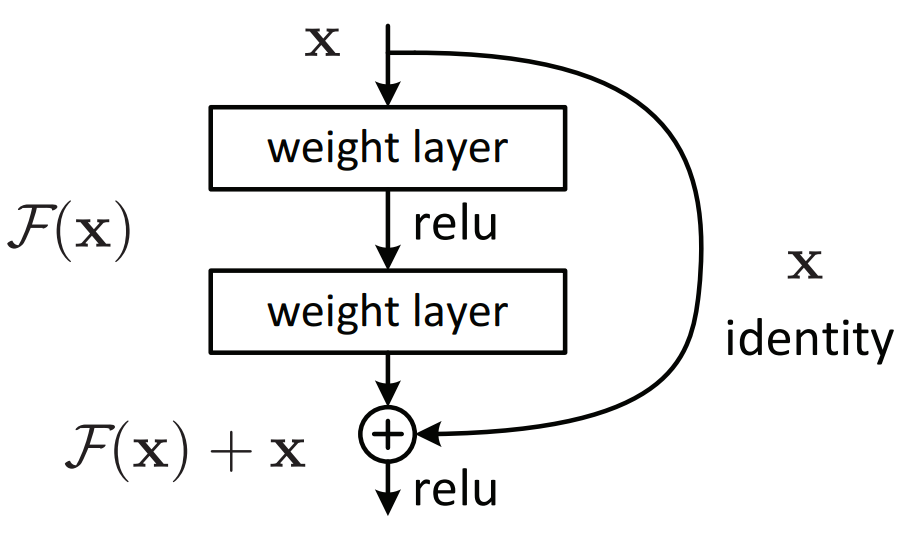
\includegraphics[width=0.4\textwidth]{images/resnet_building_block.png}
    \caption{Schema für ein Building-Block eines ResNets \cite{he2015deep}. Die
    Shortcut-Connection ist die Identität von dem Eingabeparameter $x$.}
    \label{fig:resnet-building-block}
\end{figure}

\section{Feature-Pyramid-Networks}
Bei der Objekterkennung ist beim Erlernen der Features eines Bildes die
Auflösung dieser Features sehr gering. Feature-Pyramid-Networks (FPN) haben die
Aufgabe, eine hohe Semantik bei einer hohen Auflösung zu generieren. Häufig sind
diese Netzwerke nur Teil eines Backbones bzw. werden dahinter geschaltet. Als
Backbone-Modell kann zum Beispiel AlexNet, MobileNet und ResNet dienen. In
Kombination mit einem FPN werden diese Netze damit zu einem Feature-Extractor
umgewandelt, der eine hohe Semantik bei einer hohen Auflösung der Features
erlernen kann. Der Weg von der Eingabe über das Backbone-Modell wird auch als
\textit{Bottom-Up-Pathway} bezeichnet, während der Weg vom Backbone über die
Feature-Pyramid als \textit{Top-Down-Pathway} bezeichnet wird
\cite{lin2017feature}.

Anfänglich wurden FPNs in Verbindung mit ResNet-Backbones eingeführt (siehe
Abbildung \ref{fig:resnet-fpn}). Die Eingabe ist ein $224 \times 224 \times 3$
Bild und wird mithilfe der ersten ResNet-Schicht (C1) in $112 \times 112 \times
64$ Filter mithilfe eines Convolutional-Layers mit einem Stride von 2 und einem
$7 \times 7$ Kernel umgeformt. Anschließend wird die Ausgabe in ein
Max-Pooling-Block gegeben, welcher die Eingabe in $56 \times 56 \times 128$
Filter umwandelt. Die nächsten Blöcke sind für die Einbettung von FPNs am
wichtigsten. Der folgende Block (C2) besteht aus mehreren Residual-Blocks,
welche zusammen einen Stride von 1 ergeben und 256 Filter erzeugen. Diese Blöcke
werden zusammengefasst auch \textit{Bottlenecks} genannt. Darauf folgen drei
weitere Bottleneck-Blöcke (C3, C4, C5) mit einem Stride von 2. Nach C5 ensteht
somit eine Ausgabe von $7 \times 7 \times 2048$. Soweit zum Aufbau des
Bottom-Up-Pathways. Der Top-Down-Pathway wird mithilfe von Verbindungsschichten
(Laterals) mit dem Backbone verbunden. Diese haben die Aufgabe, die Anzahl der
Filter aus dem Bottom-Up-Pathway zu umzuformen, sodass diese im Top-Down-Pathway
miteinander addiert werden können. Hierfür werden Convolutional-Layer mit einem
$1 \times 1$ Kernel und 256 Filtern verwendet, sodass lediglich die Anzahl der
Filter transformiert werden. Im Konkreten bedeutet dies, dass die Ausgabe von C5
von $7 \times 7 \times 2048$ auf die Form $7 \times 7 \times 256$ gebracht wird.
Die Größe dieser Ausgabe wird nun mithilfe von Upsampling (M5) verdoppelt und
mit der Ausgabe der Lateralverbindung von C4 addiert (M4). Dies wird mit den
übrigen Lateralverbindungen und Bottleneck-Blöcken verkettet wiederholt, sodass
das FPN schließlich vier Ausgaben mit den Größen $56 \times 56 \times 256$, $28
\times 28 \times 256$, $14 \times 14 \times 256$ und $7 \times 7 \times 256$
(M5, M4, M3, M2) ausgibt. Das Problem beim Vergrößern der Filter ist, dass dabei
ein Alias-Effekt auftritt, das Bild also verschwommen wirkt. Hierfür dienen
Smoothing-Layer, welche wiederum nichts weiter als Convolutional-Layer mit einem
$3 \times 3$ Kernel und einem Stride von 1 sind. Entsprechend werden die
Ausgaben M5 - M2 geschärft und ergeben Features mit einer hohen Auflösung und
einer hohen Semantik, die nun wahlweise für die Objekterkennung verwendet werden
können.

\begin{figure}
    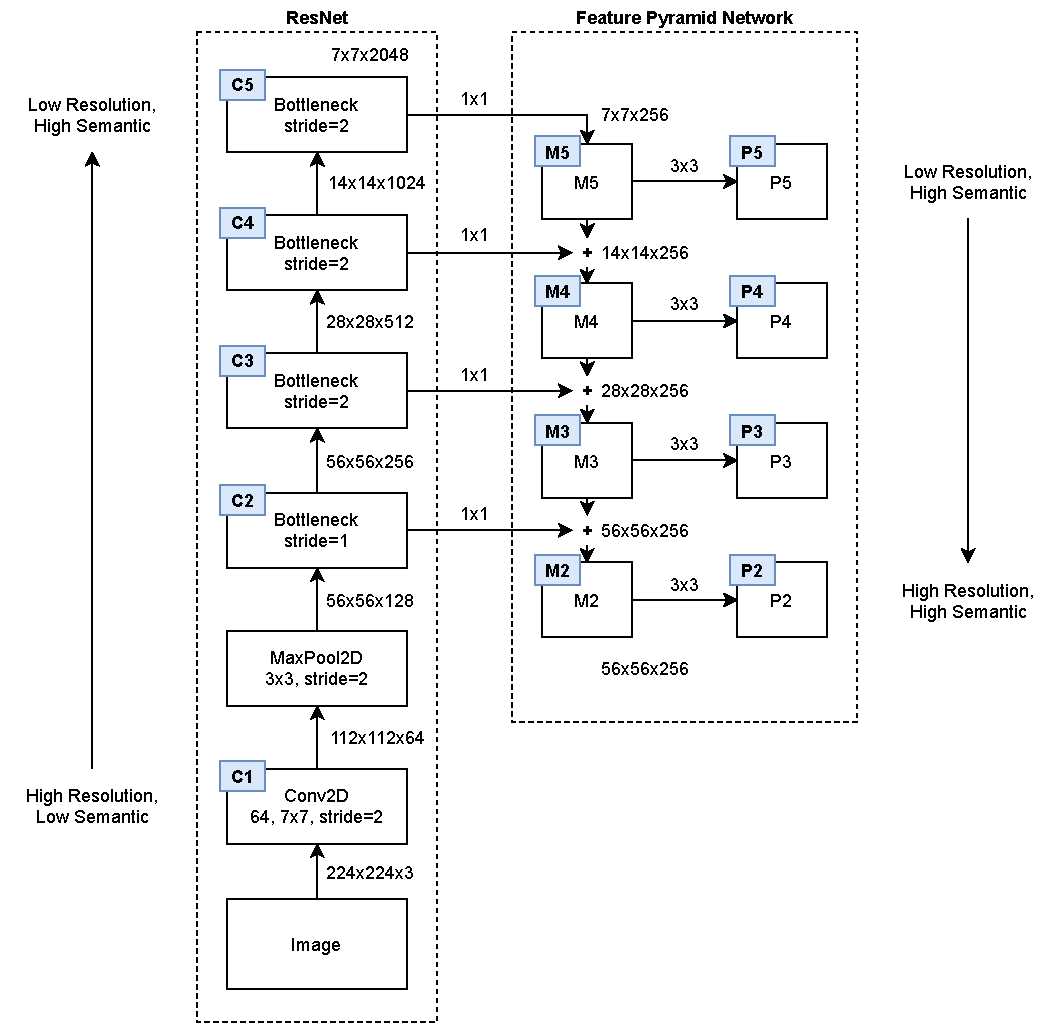
\includegraphics[width=\textwidth]{images/ResNet_FPN.pdf}
    \caption{Architektur eines Feature-Extractors als Feature-Pyramid-Network
    mit ResNet als Backbone.}
    \label{fig:resnet-fpn}
\end{figure}
  \section{Generative-Adversarial-Networks}\label{chapter:gans}
In Machine-Learning existieren viele verschiedene Modelle, die vorhandene
Datensätze analysieren und anhand der Daten lernen, Strukturen in den
Datensätzen zu erkennen.  Besitzt man beispielsweise einen Datensatz
bestehend aus Fotoaufnahmen von Tieren, so kann ein Klassifizierer trainiert
werden, um einem Bild eine Tierklasse zuzuweisen. Aus diesem Grund fässt man
diese Modelle unter dem Begriff \textit{Bildklassifizierung} \cite{lorente2021image} zusammen.

Auch interessant ist das Erkennen von vielen Objekten innerhalb eines
Bildes, anstatt das gesamte Bild nur einer einzigen Klasse zuzuweisen. In der
\textit{Objekterkennung} entwickelt man Modelle, welche mehr als nur eine
Klasse erkennen können. Sie liefern zusätzlich zu den erkannten Klassen ihre
Position und Größe innerhalb des Bildes. Diese Modelle treffen also keine
Aussage über das Gesamtbild, sondern treffen Aussagen über einzelne Objekte
innerhalb des Bildes \cite{zaidi2021survey}.

Neben Modellen, die zu einem bestimmten Sachverhalt eine Aussage treffen
können, existieren auch Modelle, welche in der Lage sind, neue Sachverhalte zu
erzeugen. Diese fallen unter dem Begriff \textit{Generative Adversarial
Networks} (GANs) und bilden das Hauptthema dieses Abschnitts. Das interessante
an diesen generativen Modellen ist, dass sie nicht nur die Strukturen eines
Datensatzes lernen, sondern darüber hinaus neue Elemente der
Ausgangsdistribution erzeugen können. Trainiert man also ein generatives
Modell auf einen Datensatz, welcher Bilder von verschiedenen Tieren enthält,
können neue Bilder der gleichen Art erzeugt werden.

Aber nicht nur zum Erzeugen von Bildern kann diese Art von Modellen verwendet
werden. Auch bei Aufgaben, bei denen eine Voraussagung getroffen werden soll,
werden generative Modelle eingesetzt. Beispielsweise wurde in
\cite{barsoum2017hpgan} gezeigt, wie zu bereits getätigten menschlichen
Bewegungen unterschiedliche, darauf folgende Bewegungssequenzen aussehen
können. Hier hat man also versucht, eine Vorhersage zur Entwicklung von
menschlichen Bewegung zu tätigen.

Die Funktionsweise von GANs ist im Prinzip ziemlich simpel. Während beim
klassischen überwachten Lernen (Supervised-Learning) in der Regel nur ein
Modell beim Training involviert ist, verhält sich das bei generativen Modellen
etwas anders. Zum Einen wird ein Generator definiert, welcher, wie sein Name
andeutet, Ausgaben selbst erzeugt. Zum Anderen wird ein Diskriminator in das
Training eingebaut, welcher zwischen künstlich erzeugten und realen Daten
unterscheidet. Diese beiden Modelle werden dann gleichermaßen trainiert.
Während der Generator versucht, immer bessere Fälschungen zu erzeugen, versucht
der Diskriminator immer besser zwischen Fälschung und Realität zu
unterscheiden. Die Ausgabe des Diskriminators ist dementsprechend entweder 0
für Fälschung und 1 für Realität. Mit anderen Worten, die beiden Komponenten
spielen ein Spiel, in welchem die eine Partei versucht, die andere zu täuschen
und wird mithilfe des folgenden Ausdrucks definiert \cite{goodfellow2014generative}.
\[
\min_G \max_D V(G, D) = \mathbb{E}_{x \sim p_{data}(x)}\left[ \log D(x) \right] + \mathbb{E}_{z \sim p_z(z)}\left[ \log (1 - D(G(z))) \right]
\]

Der Eingabeparameter $z \in \mathbb{R}^n$ stellt einen $n$-dimensionalen Vektor
dar, welcher auch als latenter Vektor bezeichnet wird. Dementsprechend wird der
Vektorraum auch als latenter Raum bezeichnet. Ein solcher Vektor repräsentiert
verschiedenste Objekte mithilfe seiner $n$ Komponenten. In Bezug zu GANs wurde
festgestellt, dass ein GAN nicht nur lernt ähnliche Daten zu einem bestehenden
Datensatz zu erzeugen, sondern auch den Zusammenhang zwischen den latenten
Komponenten und der Ausgabe zu verstehen. Das schöne daran ist, dass diese
latenten Vektoren mithilfe der Gesetze aus der linearen Algebra analysiert und
entsprechende Operationen mit ihnen ausgeführt werden können. Hierzu kann
folgendes, sehr einfaches Experiment durchgeführt werden. Man wählt zwei
latente Vektoren $a, b \leftarrow \mathbb{R}^n$, wobei die Komponenten dieser
Vektoren gleich sind, also $a_i = b_i, \; 0 \leq i < n$. Nun wählt man einen
zufälligen Komponentenindex $j \in \mathbb{N}$ mit $j \in \left[0, n\right[$
und wählt einen zufälligen Wert für die Komponenten beider Vektoren $a_j
\leftarrow \mathbb{R},\; b_j \leftarrow \mathbb{R}$, wobei $a_j \neq b_j$.
Betrachtet man nun die Ausgaben des Generators mit $a$ und $b$ als Eingabe,
dann unterscheiden sich diese um die Eigenschaft, die durch die Komponente an
der Stelle $j$ beeinflusst wird. Das gleiche Prinzip kann auch rückwärts
durchgeführt werden. Erzeugt der Generator zum Beispiel ein Bild, worauf ein
Gesicht mit Brille zu sehen ist und ein weiteres Bild mit Gesicht ohne
Brille, dann kann man die beiden Eingabevektoren voneinander subtrahieren und
damit die Komponenten herausfinden, die für die entsprechenden Eigenschaften
zuständig sind (in diesem Fall, ob das Gesicht eine Brille trägt oder nicht).

Im Verlauf des Trainings entwickelt sich damit ein Generator, welcher im
Idealfall so gute Fälschungen erzeugt, sodass sich diese nicht mehr von Daten
der Ausgangsdistribution unterscheiden lassen. Der Diskriminator kann hier
bestenfalls nur raten, also eine Genauigkeit von höchstens 50\%
erreichen. Ist dies nicht der Fall, d.h. der Diskriminator kann Fälschungen
mit einer höheren Wahrscheinlichkeit von realen Daten unterscheiden, so
entsteht ein Ungleichgewicht. Aus diesem Grund sollten die Lernparameter
sorgfältig ausgewählt und untersucht werden, damit ein stabil laufendes GAN
trainiert wird.

\subsection{Das Mode-Collapse-Problem}
Ein großes Problem beim Trainieren von generativen neuronalen Netzen ist, dass
sich der Generator sehr häufig auf bestimmte Merkmale der Ausgangsdistribution
des Datensatzes fixiert. Das Ergebnis sind signifikant erhöht wiederkehrende
Ergebnisse, die sich kaum bis gar nicht von anderen Ausgaben unterscheiden.
Man erwartet jedoch, dass das jeweilige GAN eine vielseitige Variation aus
allen Elementen des Datensatzes erzeugt. Mit anderen Worten, bei einer
zufälligen Eingabe in das Netz, soll immer eine unterschiedliche Ausgabe
erzeugt werden. Bei einem Mode-Collapse ist dies nicht der Fall. Es kann
beispielsweise passieren, dass wenn das Netz auf das Erzeugen von neuen
Gesichtern trainiert wird, dieses ausschließlich weibliche Gesichter
erzeugt. Das Netz könnte herausgefunden haben, dass es einfacher ist, weibliche
Gesichtszüge zu generieren, als männliche \cite{richardson2018gans}. Dies
lässt sich damit erklären, dass der Generator beim Trainingsvorgang mehr
Erfolg beim Generieren von weiblichen Gesichtern hatte und der Diskriminator
es schwerer hatte, Fälschung von Realität zu unterscheiden. Um das Problem zu
beseitigen wurden einige Änderungen an dem Standardmodell des GAN von
\cite{goodfellow2014generative} vorgenommen. Wie dieses Problem gelöst wird,
soll in den nächsten Abschnitten erläutert werden.

\subsection{Deep-Convolution-GAN}
Das \textit{Deep-Convolution-GAN} (DCGAN) ist ein Versuch,
\textit{Convolutional-Neural-Networks} (CNNs) mit GANs zu verknüpfen. Nach
vielen Fehlschlägen in der Entwicklung von GANs mit CNNs ist die Version von
\cite{radford2016unsupervised} stabil und auf viele unterschiedliche
Datensätze anwendbar. Dafür wurden viele verschiedene Kombinationen von
Schichten untersucht und es wurde dabei eine Architektur ausgearbeitet, die
in ein stabiles Training über verschiedenste Datensätze resultierte.
Zusätzlich können mithilfe dieser Architektur höhere Auflösungen und tiefere
Netze erreicht werden.

Zusätzlich zur eigentlichen Architektur von DCGAN werden moderne Techniken
verwendet, um CNN-Architekturen zu vereinfachen.  Damit der Generator über
mehrere Schichten hinweg die räumliche Darstellung von Objekten lernen kann,
werden Convolutional-Layer verwendet. Anstelle von sogenannten
Max-Pooling-Layer können nach \cite{springenberg2015striving} einfach
Convolutional-Layer mit erhöhtem Stride verwendet werden, ohne dass die
Genauigkeit sinkt. In Bezug zu DCGANs von \cite{radford2016unsupervised} werden
solche Schichten verwendet, um dem Generator das Erlernen vom räumlichen
Upsampling zu ermöglichen. Auch der Diskriminator wird mit solchen CNN-Layer
ausgestattet, um räumliches Downsampling zu erlernen.

Neben dem Auslassen von Max-Pooling-Layer folgt DCGAN auch dem Trend,
Fully-Connected-Layer nach jedem Convolutional-Layer zu vermeiden. Dabei
wurde festgestellt, dass die Verknüpfung von Fully-Connected-Layer und der
Eingabe des Generators bzw. mit der Ausgabe des Diskriminators am besten
funktionieren. Die erste Schicht des Generators ist also ein
Fully-Connected-Layer (1-dimensional), jedoch wird die Ausgabe der Schicht in
einen 4-dimensionalen Tensor umgewandelt. Im Falle des Diskriminators wird die
Ausgabe des letzen Convolutional-Layers (4-dimensional) abgeflacht und in eine
1-dimensionale Fully-Connected-Schicht mit einer Sigmoid-Aktivierungsfuntion gegeben.
\cite{radford2016unsupervised}.

Um Mode-Collapse zu vermeiden, verwendet \cite{radford2016unsupervised}
Batch-Normalisierungsschicht. Dadurch wird das Training stabilisiert und Probleme
wie \textit{Internal-Covariate-Shifting} angegangen \cite{pmlr-v37-ioffe15}.
Vor allem wird dadurch aber auch verhindert, dass der Generator immer die
gleichen Ausgaben erzeugt. Das Anwenden der Batch-Normalisierung in allen
Schichten des Netzwerks führt jedoch zur Stichprobenoszillation und
Instabilität des Modells. Aus diesem Grund wird auf Batch-Normalisierung in der
Ausgabesschicht des Generators und in der Eingabeschicht des Diskriminators
verzichtet.

Als letzte Beobachtung stellt \cite{radford2016unsupervised} fest, dass das
Hinzufügen von ReLU-Ak\-ti\-vier\-ungs\-funk\-tio\-nen in allen Schichten des
Generators zu schnellerem Lernen und Abdeckung der Farbräume der
Trainingsdistribution führt. In der Ausgabeschicht wird jedoch anstatt von
ReLU-Aktivierung eine Tanh-Aktivierung verwendet. Innerhalb des Diskriminators
werden schließlich Leaky-ReLU-Aktivierungen angewandt.

\begin{figure}
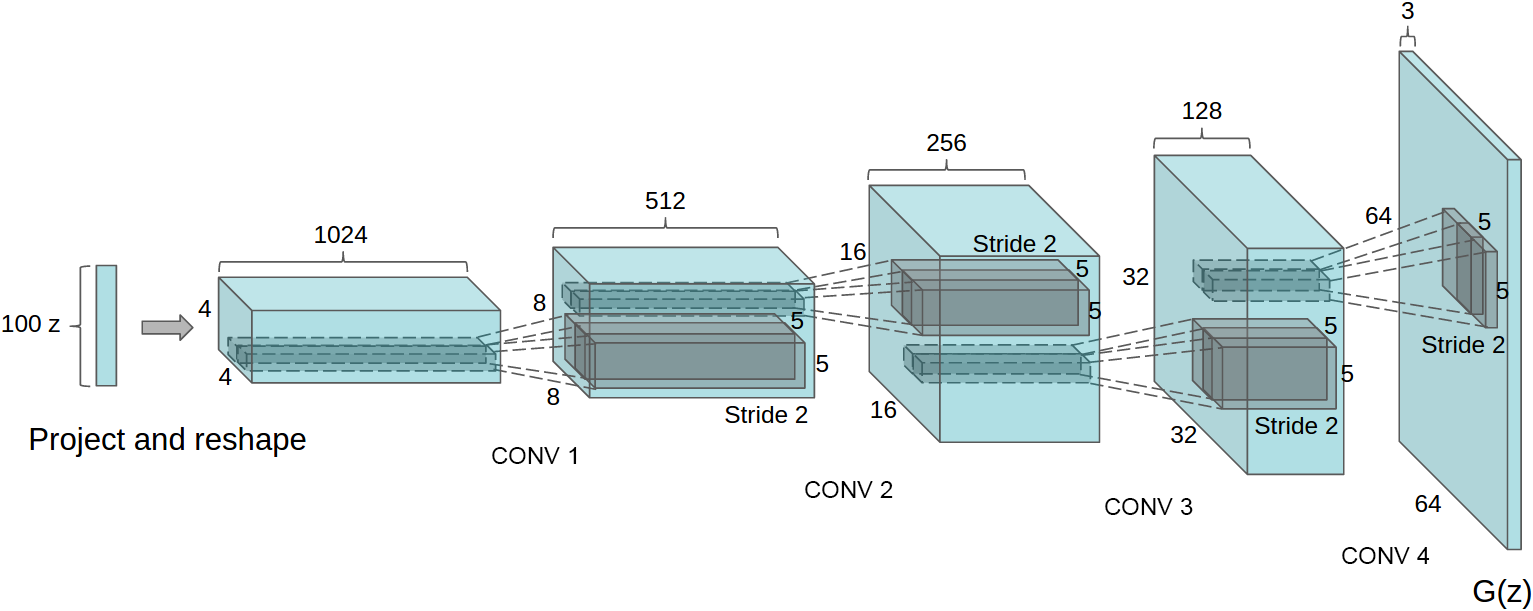
\includegraphics[width=\textwidth]{images/dcgan-architecture}
\caption{DCGAN-Architektur des Generators von
\cite{radford2016unsupervised}. Als Eingabe dient ein 100-dimensionaler
Vektor, dessen Elemente zufällig gewählt werden. Dieser wird dann in den
ersten Schichten umgeformt und durch vier Convolutional-Layer auf die Form
3$\times$64$\times$64 gebracht. Die Strides geben dabei den
Vergrößerungsfaktor pro Convolution-Schicht an, während die Anzahl der
Filter den Farbkanälen entsprechen.}
\end{figure}

\subsection{Wasserstein-GAN}
Anders als andere GAN-Varianten verwendet das Wasserstein-GAN (WGAN) die
Was\-ser\-stein-Distanz anstelle der JS- oder KL-Divergenz, um die Gewichte
von generativen neuronalen Netzen zu optimieren. Da sich die Berechnung aller
möglichen gemeinsamen Verteilungen $\gamma \sim \Pi(P_r, P_\theta)$ etwas schwierig
gestaltet, formt \cite{arjovsky2017wasserstein} die Definition unter
Berücksichtigung der Kontorovich-Rubinstein-Dualität um, sodass
\[
W(P_r, P_\theta) = \sup_{\|f\|_L \leq 1} \mathbb{E}_{x \sim P_r}\left[f(x)\right] - \mathbb{E}_{x \sim P_\theta}\left[f(x)\right]
\]

gilt, wobei das Supremum über alle 1-Lipschitz-Funktionen $f : X \to
\mathbb{R}$ ist. Zusätzlich wird ein kleiner Trick angewandt, um das Problem
weiter zu vereinfachen, indem K-Lipschitz-kontinuierliche Funktionen verwendet
werden.
\[
K \cdot W(P_r, P_\theta) = \sup_{\|f\|_L \leq K} \mathbb{E}_{x \sim P_r}\left[f(x)\right] - \mathbb{E}_{x \sim P_\theta}\left[f(x)\right]
\]

Nehmen wir nun an, dass die Abbildung $f \in \left\{f_w\right\}_{w \in W}$
parametrisiert durch $w$ existiert, wobei $W$ die Menge aller möglichen
Parameter darstellt, so können die Parameter $w$ und damit die Abbildung $f_w$
von einem neuronalen Netz erlernt werden, um so die Wasserstein-Distanz
effizient abzuschätzen. Hier bildet der Wasserstein-Abstand also gleichzeitig
die Verlustfunktion des Kritisierer mit
\[
W(P_r, P_\theta) = \max_{w \in W} \mathbb{E}_{x \sim P_r}\left[f_w(x)\right]
- \mathbb{E}_{z \sim P_r(z)}\left[f_w(g_\theta(z))\right].
\]

Trotzdem darf nicht vergessen werden, dass dies nur gültig ist, falls die
Funktion 1-Lipschitz-kontinuierlich ist. Um dies zu erzwingen, werden die
Werte der aktualisierten Gewichte des Kritisierer zwischen $\left[-c; c\right]$
gehalten. Dabei muss laut \cite{arjovsky2017wasserstein} $c$ relativ klein
sein.

\begin{algorithm}
\SetAlgoLined
\KwIn{Lernrate $\alpha$, Clipping-Parameter $c$, Batch-Größe
$m$, Anzahl von Kritisierer-Iterationen $n_{critic}$.}
\KwResult{Trainieren der Kritisierer-Parameter
$w$ und Generator-Parameter $\theta$.}
\caption{Wasserstein GAN nach \cite{arjovsky2017wasserstein}. Standardwerte
für die Eingabeparameter sind $\alpha = 5\cdot10^{-5}, c = 0.01, m = 64$
und $n_{critic} = 5$.}
\label{alg:wgan}
\BlankLine

\While{$\theta$ \textnormal{ist nicht konvergiert}}{
    \For{$t = 0, ..., n_{critic}$}{
    Erzeuge Batch $\left\{x_i \;\lvert\; 1 \leq i \leq m\right\} \sim
    \mathbb{P}_r$ aus realen Daten\;
    Erzeuge Batch $\left\{z_i \;\lvert\; 1 \leq i \leq m\right\} \sim
    \mathbb{P}_z$ aus latenten Vektoren\;
    \BlankLine
    $g_w \leftarrow
    \nabla_w \left[ \frac{1}{m}\sum_{i=1}^{m} f_w(x_i) -
    \frac{1}{m}\sum_{i=1}^{m} f_w(g_\theta(z_i)\right]$\;
    \BlankLine
    $w \leftarrow w + \alpha \cdot \mathrm{RMSProp}(w,
    g_w)$\;
    $w \leftarrow \mathrm{clip}(w, -c, c)$\;
    }
    \BlankLine
    Erzeuge Batch $\left\{z_i \;\lvert\; 1 \leq i \leq m\right\} \sim
    \mathbb{P}_z$ aus latenten Vektoren\;
    $g_\theta \leftarrow -\nabla_\theta \left[\frac{1}{m} \sum_{i=1}^{m}
    f_w(g_\theta(z_i))\right]$\;
    $\theta \leftarrow \theta - \alpha \cdot \mathrm{RMSProp}(\theta,
    g_\theta)$\;
}
\end{algorithm}

Zusätzlich ist bei Wasserstein-GANs von einem Kritisierer (Critic) anstatt
eines Diskriminators die Rede. Der Grund dafür ist, dass ein Diskriminator
zwischen \textit{fake} und \textit{real} unterscheidet, mehr nicht. Der
Kritisierer führt diese Unterteilung der Eingabeparameter nicht durch, sondern
bewertet bzw. kritisiert diese viel mehr. Mathematisch ausgedrückt sprechen
wir hierbei von einer linearen Ausgabe in $\mathbb{R}$ im Falle des
Kritisierers, während der Diskriminator eine binäre Ausgabe erzeugt.  Zu
Beginn von Algorithmus \ref{alg:wgan} werden die Parameter $w$ für den
Kritisierer und $\theta$ für den Generator initialisiert. Anschließend werden
$m$ Datenpunkte bzw. ein Batch aus dem reellen Datensatz (Verteilung
$\mathbb{P}_r$) gezogen. Dies muss nicht unbedingt zufällig sein. Auch werden
$m$ zufällige Vektoren erzeugt, die als Eingabe für den Generator dienen,
welcher wiederum Fake-Daten erzeugt. Dabei bilden die Ausgaben des Generators
eine eigene Verteilung $\mathbb{P}_\theta$.  Ziel des Generators ist es nun,
die Distanz zwischen den beiden Verteilungen $\mathbb{P}_r, \mathbb{P}_\theta$
zu minimieren, um möglichst realitätsnahe Ausgaben erzeugen zu können. Als
nächstes werden die Gradienten $g_w$ für Parameter $w$ mithilfe von
Gradient-Descent, dargestellt als $\nabla_w$, berechnet. Hierfür wird die
Wasserstein-Distanz als Verlustfunktion verwendet.  Der nächste Schritt besteht
daraus, die Parameter $w$ des Kritisierer-Netzwerks mithilfe des
RMSprop-Algorithmus zu aktualisieren und die aktualisierten Gewichte so gering
wie möglich zu halten, um die K-Lipschitz-Kontinuität zu gewährleisten. Dies
wird mithilfe der Funktion \textit{clip} umgesetzt, welche die
Parameterwerte in einem bestimmten Intervall $\left[-c; c\right]$ festsetzt.
Die bis hier erläuterten Schritte werden $n_{critic}$-mal durchgeführt, sodass
das Kritisierer-Netzwerk immer öfter trainiert wird, als der Generator. Dieser
wird nun optimiert, indem wieder $m$ Vektoren zufällig erzeugt und als Eingabe
für das Generator-Netzwerk verwendet werden. Der Generator erzeugt damit $m$
zufällige Ausgaben, die wiederum als Eingaben in das Kritisierer-Netzwerk
gegeben werden. Aus den Ausgaben wird dann der Mittelwert gebildet und zum
Bestimmen der Gradienten von den Generator-Parametern $\theta$ verwendet.

Im direkten Vergleich zu dem originalen GAN \cite{goodfellow2014generative}
werden einige Änderungen in der Architektur vorgenommen. Während in dem
originalen Anstatz fast nach jeder Schicht eine Batch-Normalisierung
vorgenommen wird, können diese bei WGANs entfallen. Standard-GANs würden
hierbei kaum interpretierbare Resultate erzeugen, WGANs hingegen produzieren
trotzdem gute Ergebnisse, wie Experimente von \cite{arjovsky2017wasserstein}
zeigen (siehe Abbildung \ref{fig:wgan-gan-no-batchnorm}). Das Wasserstein-GAN
hat zusätzlich noch einige nützliche Eigenschaften. So wird unter anderem
durch Annäherung des Wasserstein-Abstandes zwischen Generator- und
Ausgangsdistribution das Problem des Mode-Collapse gelöst.  Durch den
Wasserstein-Abstand wird der Abstand zwischen den Verteilungen wesentlich besser
minimiert als bei der KL- oder JS-Divergenz.
Die Ausgabe eines Kritisierers stellt außerdem eine Bewertung der Eingabe dar,
anstatt diese in die Kategorien Fälschung oder Realität einzuteilen und besitzt
deshalb mehr Aussagekraft.

\begin{figure}
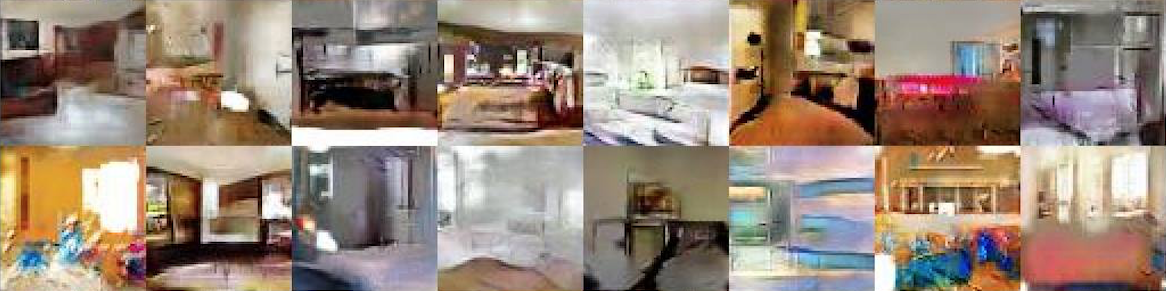
\includegraphics[width=0.5\textwidth]{images/image-022.png}

\includegraphics[width=0.5\textwidth]{images/image-024.png}
\caption{Vergleich von WGAN und Standard-GAN \cite{arjovsky2017wasserstein}.
    Links sind Ausgaben vom WGAN-Algorithmus zu sehen, während rechts Ausgaben
    eines Standard-GANs dargestellt sind. In beiden Generator-Modellen wurden
    Batch-Normalisierungsschicht entfernt. Klar zu erkennen ist, dass WGAN immer
    noch interpretierbare Ergebnisse liefert, während bei Standard-GANs Probleme
    erkennbar sind.}
\label{fig:wgan-gan-no-batchnorm}
\end{figure}

\subsection{Wasserstein-GAN mit Gradient-Penalty}
Ein großes Problem von Wasserstein-GANs ist das Abschneiden der
Netzwerkgewichte (Weight-Clipping) in ein fest definiertes Intervall, um die
1-Lipschitzstetigkeit zu erfüllen. Das dies keine elegante Lösung ist, liegt
auf der Hand. In \cite{gulrajani2017improved} wurde speziell dieses Problem
genauer untersucht und es wurde festgestellt, dass das Beschneiden der Gewichte
den Kritisierer dazu verleitet, nur extrem einfache Funktionen zu erlernen, wie
der Vergleich in Abbildung \ref{fig:problems-of-weight-clipping} zeigt. 

Um das Problem mit dem Abschneiden der Gewichte anzugehen, stellt
\cite{gulrajani2017improved} eine alternative Lösung vor, die auf anderem Wege
die 1-Lipschitzstetigkeit in WGANs sicherstellen soll. Hierbei soll
Gradient-Penalty helfen und wird als
\[
(\|\nabla_{\hat{x}} D(\hat{x})\| - 1)^2
\]
berechnet, wobei $\hat{x} =  x \epsilon + \tilde{x}(1 - \epsilon)$ eine
zufällige Gewichtung zwischen realen ($x$) und generierten Daten ($\tilde{x}$)
darstellt. Das $\epsilon$ wird dabei zufällig aus $\left[0, 1\right]$ gewählt.
Daraus resultierend gestaltet sich die neue Verlustfunktion des Kritisierers wie
folgt.
\[
L = \mathbb{E}_{\tilde{x} \sim \mathbb{P}_g}\left[D(\tilde{x})\right] -
    \mathbb{E}_{x \sim \mathbb{P}_r}\left[D(x)\right] +
    \lambda \cdot \mathbb{E}_{\hat{x} \sim \mathbb{P}_{\hat{x}}}\left[(\|\nabla_{\hat{x}} D(\hat{x})\| - 1)^2\right]
\]
Der Kritisierer ist durch diese Änderung nun wesentlich besser dazu in der
Lage, komplexere Verteilungen zu erlernen.

\begin{algorithm}
\caption{WGAN mit Gradient-Penalty \cite{gulrajani2017improved}.}
\KwIn{Gradient-Penalty-Koeffizient $\lambda$, Anzahl von Kritisierer-Iterationen
$n_{critic}$, Batch-Größe $m$, Adam-Hyperparameter $\alpha, \beta_1,
\beta_2$.}
\KwResult{Trainieren der Kritisierer-Parameter $w$ und Generator-Parameter
$\theta$.}
\BlankLine
\While{$\theta$ \textnormal{ist nicht konvergiert}}{
    \For{$t = 1, ..., n_{critic}$}{
    \For{$i = 1, ..., m$}{
        Wähle reale Probe $x \sim \mathbb{P}_r$, latenten Vektor $\vec{z} \sim
        \mathbb{P}_z$, zufällige Zahl $\epsilon \in \left[0, 1\right]$\;
        $\tilde{x} \leftarrow G_\theta(\vec{z})$\;
        $\hat{x} \leftarrow x\epsilon + \tilde{x}(1 - \epsilon)$\;
        $L_i = D_w(\tilde{x}) - D_w(x) + \lambda(\|\nabla_{\hat{x}}
        D_w(\hat{x})\| - 1)^2$\;
    }
    \BlankLine
    $w \leftarrow \mathrm{Adam}(\nabla_w \frac{1}{m} \sum_{i=1}^m L_i, w,
    \alpha, \beta_1, \beta_2)$\;
    }
    \BlankLine
    Wähle einen Batch aus latenten Vektoren $\{\vec{z}_i\}_{i=1}^m \sim
    \mathbb{P}_z$\;
    $\theta \leftarrow \mathrm{Adam}(\nabla_{\theta} \frac{1}{m} \sum_{i=1}^m
    - D_w(G_\theta(\vec{z}_i)), \theta, \alpha, \beta_1, \beta_2)$\;
}
\end{algorithm}

\begin{figure}
\centering
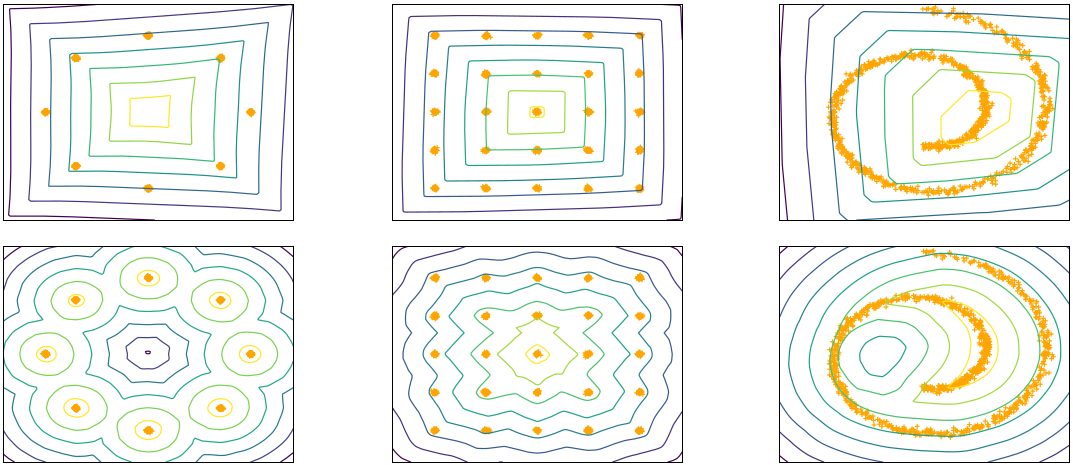
\includegraphics[width=\textwidth]{images/problems_of_weight_clipping}
\caption{Vergleich zwischen Weight-Clipping (oben) und Gradient-Penalty
(unten). Man erkennt deutlich, dass die Separierung der Ausgangsverteilung,
dargestellt durch orangene Punkte, durch Weight-Clipping in sehr
vereinfachte Funktionen resultiert. Gradient-Penalty lässt hingegen
komplexere Strukturen von Verteilungen zu \cite{gulrajani2017improved}.}
\label{fig:problems-of-weight-clipping}
\end{figure}

\subsection{Conditional-Wasserstein-GAN mit Gradient-Penalty}\label{section:cwgan-gp}
Generative Modelle wie das WGAN oder DCGAN erzeugen bei einem zufälligen
Eingabevektor immer ein zufälliges, interpoliertes Element aus der
Trainingsdistribution. Besitzt der Trainingsdatensatz verschiedene Klassen, so
werden diese Modelle auch zwischen den Klassen interpolierte Ergebnisse
erzeugen. Aber was ist, wenn wir ein zufälliges Element einer bestimmten Klasse
erzeugen wollen? Nehmen wir als Beispiel einen Datensatz bestehend aus Bildern
von Hunden und Katzen. Die bisher vorgestellten DCGANs und WGANs würden auf
diesen Datensatz trainiert werden und würden bei einem zufälligen Eingabevektor
Hunde oder Katzenbilder bzw. eine Mischung aus beidem erzeugen. Möchte man nun
jedoch den Generator des GANs dazu bringen, nur zufällige Hundebilder zu
erzeugen, so muss aufwändig die dafür zuständige Komponente des Eingabevektors
extrahiert werden, die bestimmt, ob der Generator ein Hunde- oder ein Katzenbild
erzeugen soll. Eine einfachere Möglichkeit besteht darin, dem Generator
zusätzlich zum latenten Vektor die Klasse der zu erzeugenden Ausgabe zu
übergeben. Diese Idee wurde erstmals mit
Conditional-Generative-Adversarial-Networks (cGANs) \cite{mirza2014conditional}
umgesetzt und stellt eine Erweiterung zu den bisher besprochenen GANs dar.

Wie bereits erwähnt, wird bei cGANs zusätzlich zum latenten Vektor $x$ das Label
bzw. die Klasse $y$ als Eingabe verwendet. Wie dies technisch umgesetzt wird,
soll das Schema in Abbildung \ref{fig:cgan} verdeutlichen. Die beiden Eingaben,
latenter Vektor und Label, werden zuerst mithilfe einer Vollverbindungsschicht
(Dense) und Umformungsschicht (Reshape) auf die gleiche Form gebracht, da diese
nicht unbedingt gleich aufgebaut sein müssen. Anschließend werden die nun
zueinander passenden Eingaben mithilfe einer Verkettungsschicht (Concat)
aneinandergehängt. Der restliche Verlauf verhält sich wie bei den anderen
vorgestellten GANs, also das Hochskalieren der kleinen Eingabegröße mithilfe von
mehreren aneinandergereihten transponierten Faltungsschichten (Conv2D
Transpose). Die Verlustfunktion für das Trainieren des cGANs muss aufgrund der
Verkettung beider Eingaben ebenfalls angepasst werden. 
\[
\min_G \max_D V(G, D) = \mathbb{E}_{x \sim p_{data}(x)}\left[ \log D(x \lvert y) \right] + \mathbb{E}_{z \sim p_z(z)}\left[ \log (1 - D(G(z \lvert y))) \right]
\]

Die Verknüpfung $\lvert$ stellt dabei die Verkettungsoperation dar, sodass $x
\lvert y$ bedeutet, dass $y$ an $x$ gehängt wird. Aus diesem Grund müssen $x$
und $y$ auch dieselbe Form aufweisen. Andernfalls kann die Verkettung nicht
durchgeführt werden. Das komplette Netzwerk lernt damit eine Ausgabe zu
erzeugen, die auf das eingegebene Label passt. Soweit zur Idee von
Conditional-Generative-Adversarial-Networks. Dies soll nun auf Wasserstein-GANs
übertragen werden, sodass in späteren Implementationen
Conditional-Wasserstein-GANs (cWGAN) zur Verfügung stehen, um automatisiert
Datensätze zu erzeugen. Die angepasste Verlustfunktion $L_w$ für den Kritisierer,
welche die Verkettung des Labels berücksichtigt, bildet sich wie folgt.
\[
L_w = \mathbb{E}_{\tilde{x} \sim \mathbb{P}_g}\left[D(\tilde{x} \lvert y)\right] -
    \mathbb{E}_{x \sim \mathbb{P}_r}\left[D(x \lvert y)\right] +
    \lambda \cdot \mathbb{E}_{\hat{x} \sim \mathbb{P}_{\hat{x}}}\left[(\|\nabla_{\hat{x}} D(\hat{x} \lvert y)\| - 1)^2\right]
\]

Der Verlust $L_\theta$ des Generators lässt sich mit
\[
L_\theta = -\mathbb{E}_{\tilde{x} \sim \mathbb{P}_g} \left[D(\tilde{x} \lvert y)\right]
\]
berechnen.

Für ein Training, in welchem die Daten in Batches vorliegen, wird einfach der
arithmetische Mittelwert der Verluste berechnet. Zur Erinnerung, $x \sim
\mathbb{P}_r$ entspricht einer Probe $x$ aus einem realen Datensatz. Das $x$
ist damit ebenfalls real. Zudem sind $\tilde{x} = G(z \lvert y)$ und $\hat{x} =
x \epsilon + \tilde{x} (1 - \epsilon)$ generierte bzw.  interpolierte Proben.
Mithilfe dieser Verlustfunktionen kann nun ein Conditional-Wasserstein-GAN mit
Gradient-Penalty implementiert werden. Besonders wird dies im nächsten Kapitel
besprochen, wenn ein Generator zum Erzeugen von ganzen Datensätzen mit
verschiedenen Klassen umgesetzt werden soll. 

\begin{figure}
    \centering
    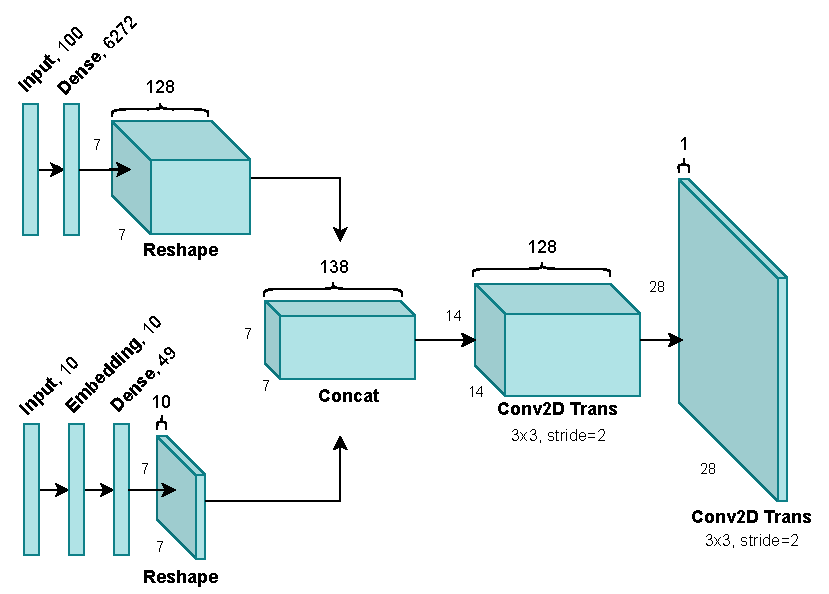
\includegraphics[width=0.8\textwidth]{images/cgan.pdf}
    \caption{Schematische Darstellung eines einfachen Conditional-GANs für den MNIST-Datensatz. Die Eingaben sind ein latenter Vektor mit 100 Komponenten und ein Labelvektor mit 10 Komponenten (entsprechend der Anzahl der Klassen).}
    \label{fig:cgan}
\end{figure}

  \chapter{Erstellen eines Datensatzes}\label{chapter:dataset}
Ein wichtiger Bestandteil beim Entwickeln von künstlichen neuronalen Netzen ist
der unterliegende Datensatz, der zum Trainieren der Parameter der Netze
verwendet wird. Eine Machine-Learning-Modell ist nur so gut wie der verwendete
Datensatz. Dieser muss deshalb eine große Varianz der repräsentierten Daten
besitzen. Das bedeutet, dass ausreichend Einträge vorhanden sein müssen, um das
Netzwerk auf ähnliche, aber unbekannte Probleme vorzubereiten. Ein beliebter
Datensatz ist beispielsweise der MNIST-Datensatz \cite{6296535}, welcher unter
anderem Bilder von handgeschriebenen Ziffern bereitstellt. Anhand des
MNIST-Beispiels bedeutet eine große Varianz, dass eine Ziffer durch viele
verschiedene Bilder repräsentiert wird, die alle eine andere Perspektive des
gleichen Kontexts darstellen.

In diesem Abschnitt soll nun ein Datensatz eingeführt werden, welcher Daten für
die Bewegungserkennung unterstützt. Um diesen Datensatz zu erstellen, muss vorab
geklärt werden, was eine Bewegung eigentlich ist. Betrachtet man einen Punkt im
Raum, dann beschreibt eine Bewegung die Änderung des Ortes eines Objekts über
die Zeit. Bezogen auf den zu erstellenden Datensatz bedeutet dies, dass einfache
Bildaufnahmen von beweglichen (dynamischen) Objekten nicht ausreichen. Um eine
Bewegung aufzuzeichnen, müssen zeitlich aufeinander folgende Bilder aufgenommen
werden, die letzlich Videos darstellen. Da der Datensatz später dazu verwendet
werden soll, um ein neuronales Netz zu trainieren, welches Bewegungen erkennt,
müssen die zu erlernenden Bewegungen auch in diesem Datensatz als Videos
vertreten sein.

Bevor ein Modell für die Bewegungserkennung und -analyse trainiert wird, soll
zusätzlich untersucht werden, ob ein relativ kleiner Datensatz ausreichend ist,
um trotzdem gute Resultate beim Trainieren von neuronalen Netzen zu erzeugen. Da
diese Netze jedoch auf einen vielseitigen Datensatz zurückgreifen müssen, um
entsprechend gute Erkennungsraten zu erzeugen, ist die Idee, diesen kleinen
Datensatz künstlich zu erweitern. Interessant hierbei ist, ob ein künstlich
gedehnter Datensatz genau so gut geeignet ist, wie ein aufwändig erstellter
Datensatz bestehend aus realen Daten. Falls sich das Experiment als erfolgreich
herausstellt, liegt der Vorteil auf der Hand. Nämlich dass künstlich erzeugte
Datensätze wesentlich schneller auszuheben sind als Datensätze mit
ausschließlich realen Daten. Dies würde den Arbeitsaufwand für das Erstellen von
neuen komplexen Datensätzen um ein vielfaches verringern und gleichzeitig den
Fokus auf die eigentliche Forschungsarbeit verbessern.

Nun stellt sich natürlich die Frage, wie ein kleiner Datensatz künstlich
vergrößert werden kann. Künstlich bedeutet hier, dass das Vergrößern des
Datensatzes mithilfe von Algorithmen geschiet und vom Computer anstatt vom
Menschen durchgeführt wird. Eine Möglichkeit ist es, die Daten zu augmentieren.
Dies wird bereits häufig während des Trainings von neuronalen Netzen
durchgeführt, indem simple Transformationen wie Rotation, Translation und
Verzerrung an den Daten durchgeführt werden. Aber auch das Verändern des
Gamma-Wertes eines Bildes reicht in einigen Fällen aus, um eine Variation im
Datensatz künstlich zu erzeugen. Eine weitere Möglichkeit ist es, anderen
neuronalen Netzen diese Arbeit übernehmen zu lassen. Hierbei werden generative
Modelle wie GANs verwendet, um neue, bisher unbekannte Samples eines Datensatzes
zu erzeugen. Auch diese Idee ist nicht neu, jedoch beziehen sich die meisten
Beispiele auf das Generieren von einfachen Bildern. Da es sich bei dem zu
erstellenden Datensatz um Videos handelt, müssen die Techniken auf dieses
Problem angewandt werden. Neben den Inhalt von einzelnen Bildern muss das GAN
als zusätzliche Dimension also die Semantik zwischen einzelnen Frames bzw.
Bildern erlernen und neu generieren können, da es keinen Sinn ergibt, dass der
Kontext pro Videoframe zufällig wechselt. Stattdessen wird gefordert, dass jeder
erzeugte Frame von dem vorherigen abhängt, sodass die Folge der Frames ein
sinnvolles Video ergibt.

\section{GAN für Videos}
In diesem Abschnitt wird die Architektur von ViGAN vorgestellt und die
Idee dahinter erläutert. ViGAN steht für Video-Generative-Adversarial-Network
und dient zum Erzeugen von neuen Videos aus einem bestehendem Datensatz. Gerade
das Erstellen von Videos und das Labeln der Bewegungen nimmt enorm viel Zeit in
Anspruch. Mithilfe von ViGAN soll der Aufwand reduziert werden. Hierbei wird
untersucht, ob ein künstlich erweiterter Datensatz für das Trainieren von
neuronalen Netzen geeignet ist. In Kapitel \ref{chapter:gans} werden
verschiedene GANs und deren Probleme bzw. Vorteile vorgestellt. Aufgrund der
Vorteile von Wasserstein-GANs, nämlich die Interpretationsmöglichkeit des Losses
während des Trainings und die Mode-Collapse-Resistenz, wird dieses als
Grundarchitektur gewählt. Da häufig GANs nur in Verbindung mit einzelnen Bildern
verwendet werden, muss das WGAN entsprechend angepasst werden, um Videos anstatt
von Bildern zu erzeugen. Wie im vorherigen Abschnitt besprochen, ist es wichtig,
dass die Frames des Videos zueinander passen und nicht aus dem Kontext gerissen
werden. Wie in Abbildung \ref{fig:vigan} dargestellt unterscheidet sich ViGAN
nicht allzu sehr vom WGAN. Der größte Unterschied besteht darin, dass
3D-Convolutional-Layer anstelle der 2D-Convolutional-Layer verwendet werden.
Dies ermöglicht nicht nur ein Upsampling des Bildes, sondern auch die Anzahl der
Frames. Die Idee dabei ist, dass das Netzwerk dadurch lernt, zusammenhängende
Frames zu generieren. Als Eingabe wird ein zufälliger Vektor $z$ gewählt. Dann
muss das Netzwerk die eindimensionale Eingabe in eine vierdimensionale Struktur
umwandeln. Dies geschieht beim ViGAN mithilfe eines Fully-Connected-Layers mit
$5 \cdot 6 \cdot 8 \cdot 256$ Neuronen und einem Reshape-Layer, welcher die
Ausgabe des Fully-Connected-Layers in einen 4D-Tensor mit den Dimensionen $(5,
6, 8, 256)$ umstrukturiert. Die erste Dimension beschreibt dabei immer die
Anzahl der Frames, die zweite die Höhe, die dritte die Breite und die vierte die
Anzahl der Farbkanäle. Anschließend wird der Tensor mithilfe eines
Convolutional-Layers vergrößert und die Frameanzahl erhöht. Der Stride beträgt
dabei 2, sodass eine Verdoppelung der Dimensionen stattfindet. Insgesamt werden
vier solcher Schichten hinereinander gereiht. Dabei entsteht ein Ausgabevideo
mit 80 Frames, wobei jeder Frame jeweils $96 \times 128 \times 3$ Pixelwerte
besitzt.

\begin{figure}
    \centering
    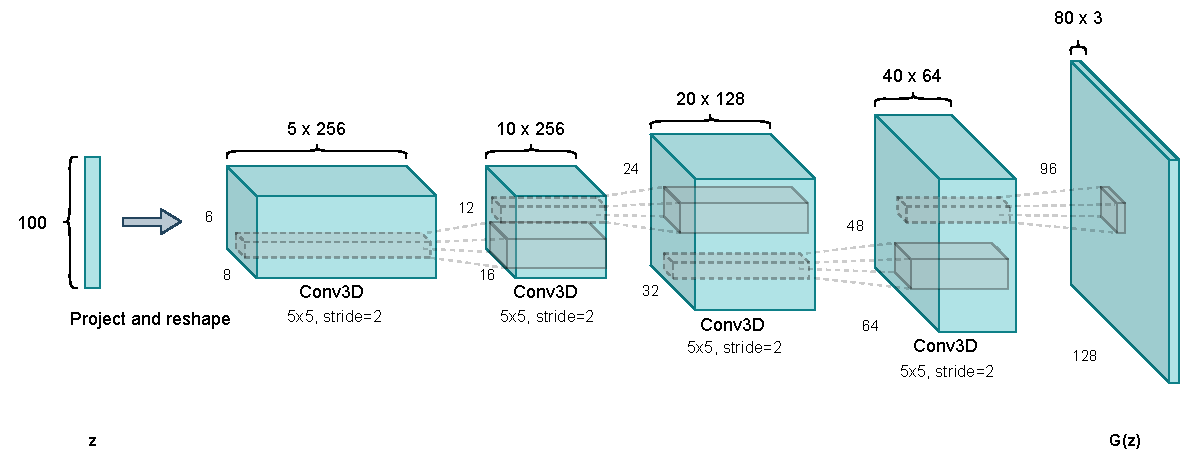
\includegraphics[width=\textwidth]{images/ViGAN.pdf}
    \caption{Architektur von ViGAN. Als Eingabe dient ein zufälliger Vektor $z
    \in \mathbb{R}^{100}$. Dieser wird anschließend in fünf $6 \times 8 \times
    256$ Features umgewandelt. Um die relativ kleinen Frames in eine größere
    Auflösung zu skalieren, werden vier 3D-Convolutional-Layer verwendet. Jedes
    dieser Schichten verwendet eine Kernelgröße von $5 \times 5 \times 5$ und
    einen Stride von 2.  Insgesamt ergibt sich also ein Stride von $2^4 = 16$,
    sodass die Eingabegröße von $5 \times 6 \times 8 \times 256$ auf 80x96x128x3
    hochskaliert wird.}
    \label{fig:vigan}
\end{figure}

\section{Training vom ViGAN}
Um ViGAN zu testen, werden einige Experimente durchgeführt, die untersuchen
sollen, ob die Ausgaben des GANs brauchbar sind. Unter anderem wird durch
Experimente herausgefunden, welcher Aufbau von Generator und Diskriminator (in
diesem Fall ist der Diskriminator ein Kritisierer) in einem stabilen Training
resultieren. Das Training wird auf eine GeForce RTX 3080 ausgelagert und dauert
im Schnitt 12 Stunden für 9000 Epochen bei einem Datensatz von 3 Videoclips mit
jeweils 840 Frames. Das größte Problem während des Trainings besteht darin, die
Trainingsdaten in den Speicher der Grafikkarte zu laden, da das Modell und die
Daten entsprechend groß sind. Daher kann nur mit einer Batch-Größe von 4
gearbeitet werden. Insgesamt wurden 8 Experimente durchgeführt, wobei sich die
Architekturen aus Tabelle \ref{table:stable-experiment} am stabilsten
herausstellten. Trotz des stabilen Trainings weisen die Ausgaben des
Generator-Netzwerkes einige Makel auf. Es entstehen zwar Videos, in denen eine
Bewegung stattfindet, jedoch sind auch Transitionen in der Inneneinrichtung
vorhanden. So verschwindet während des Videoclips beispielsweise eine Tür und es
erscheint ein Sofa. Auf jeden Fall entstehen aber Räume, die so in der Art nicht
im Datensatz vorhanden sind. Leider wird auch nicht immer eine menschliche
Bewegung erzeugt, sodass sich zwar der Raum über die Zeit ändert, die Person
aber regungslos in diesem steht.

\begin{table}
    \scriptsize
    \label{table:stable-experiment}
    \begin{tabularx}{\textwidth}{lXXXXll}
        \hline
        Input-Shape & Conv1 & Conv2 & Conv3 & Conv4 & Output-Shape & Parameter \\ \hline
        $5 \times 12 \times 16 \times 256$ & c=128 \newline s=2,2,2 & c=64 \newline s=2,2,2 & c=64 \newline s=2,2,2 & c=3 \newline s=1,2,2 & $40 \times 192 \times 256 \times 3$ & \num{3,07e7} \\ \hline

        $1 \times 3 \times 4 \times 96$ & c=96 \newline s=5,5,5 & c=48 \newline s=2,3,3 & c=16 \newline s=2,4,4 & c=3 \newline s=2,2,2 & $40 \times 360 \times 480 \times 3$ & \num{0,20e7} \\ \hline

        $1 \times 6 \times 8 \times 96$ & c=96 \newline s=5,5,5 & c=48 \newline s=3,3,3 & - & c=3 \newline s=4,4,4 & $40 \times 360 \times 480 \times 3$ & \num{0,22e7} \\ \hline

        $10 \times 20 \times 45 \times 256$ & c=128 \newline s=1,1,1 & c=64 \newline s=2,2,2 & - & c=3 \newline s=2,2,2 & $40 \times 80 \times 180 \times 3$ & \num{2,40e8} \\ \hline

        $5 \times 3 \times 4 \times 256$ & c=256 \newline s=1,1,1 & c=128 \newline s=2,2,2 & c=128 \newline s=2,2,2 & c=3 \newline s=3,3,3 & $60 \times 36 \times 48 \times 3$ & \num{1,60e7} \\ \hline

        $5 \times 3 \times 4 \times 512$ & c=256 \newline s=2,2,2 & c=128 \newline s=2,2,2 & - & c=3 \newline s=3,3,3 & $60 \times 36 \times 48 \times 3$ & \num{2,37e7} \\ \hline

        $5 \times 6 \times 8 \times 256$ & c=128 \newline s=2,2,2 & c=64 \newline s=2,2,2 & c=32 \newline s=2,2,2 & c=3 \newline s=2,2,2 & $80 \times 96 \times 128 \times 3$ & \num{1,17e7} \\ \hline

        $15 \times 12 \times 16 \times 256$ & c=128 \newline s=2,2,2 & c=64 \newline s=2,2,2 & - & c=3 \newline s=2,2,2 & $120 \times 96 \times 128 \times 3$ & \num{8,03e7} \\ \hline
    \end{tabularx}
    \caption{Experimente mit ViGAN. Es wurde untersucht, welche Konfigurationen
    zu einem stabilen Training führen. Außerdem wurde versucht, die Anzahl der
    erzeugten Frames so hoch wie möglich zu halten. Die Convolutional-Layer
    besitzen alle $5 \times 5 \times 5$ Kernels. Die Parameter $c$ und $s$ beschreiben entsprechend die Channels und Strides der Convolutional-Layer.}
\end{table}

\section{GAN für Schlüsselpunktanimationen}
Da das ViGAN einige Probleme aufgewiesen hat, wurde eine alternative Methode
entwickelt, um Bewegungen effizienter und genauer zu generieren. Auch in dieser
Methode wird ein GAN verwendet, nur diesmal wird die Information einer Bewegung
wesentlich genauer betrachtet. Das Ziel ist ein schnelleres Training des
Netzwerks sowie ein geringerer Speicherverbrauch. Ein großer Nachteil beim ViGAN
ist, dass viele unnötige Informationen mit generiert werden. Anstatt also Videos
herkömmlicher Art zu erzeugen, sollen nun Animationen bestehend aus
Schlüsselpunkten des menschlichen Körpers generiert werden. Die Folge dieser
Schlüsselpunkte soll schließlich eine Bewegung darstellen. Extrahiert man die
Schlüsselpunkte aus entsprechenden Videos, die eine Bewegungsart beinhalten, so
wird der eigentliche Datensatz um ein vielfaches reduziert, jedoch bleibt die
zu betrachtende Information gleich -- bei der Bewegungserkennung interessiert
nur die Bewegung und nicht die Umgebung. Genau wie beim ViGAN wird hier
ebenfalls ein WGAN als Grundarchitektur verwendet. Im Grunde verhält sich das
Netzwerk ähnlich, außer dass es lediglich einzelne Bilder anstatt Videos
generiert.

Eine Bewegung bestehend aus $N$ Frames und $k$ Schlüsselpunkten, welche jeweils
eine Position im zweidimensionalen Raum und eine Auftrittswahrscheinlichkeit
besitzen, können mithilfe eines Bildes repräsentiert werden. Ein solches Bild
besitzt damit eine Größe von $N \times k \times 3$. Da später Modelle verwendet
werden, welche auf dem \textit{COCO Keypoints Dataset} \cite{lin2015microsoft}
trainiert sind und 17 Schlüsselpunkte von Menschen in Bildern erkennen, wird $k
= 17$ gewählt. Zudem wird die Anzahl an Frames auf $N = 60$ gesetzt, es wird
also angenommen, dass entsprechende Bewegungen innerhalb von 60 Frames eindeutig
erkennbar sind. Die Ausgaben des GANs sind dementsprechend im Format $60 \times
17 \times 3$. In Abbildung \ref{fig:motion-images} wurden beispielhaft drei
Bewegungsarten zu Bilder kodiert und deren ersten 10 Frames dargestellt, die
durch die ersten 10 Reihen des jeweiligen Bildes repräsentiert werden. Auf Basis
dieser Bilder wird nun ein GAN entwickelt, welches neue Bewegungen des gleichen
Typs erzeugen soll. Mit anderen Worten, das GAN soll lernen, ähnliche Bilder zu
erzeugen, die wiederum in Schlüsselpunktanimationen dekodiert werden können.
Wenn dieses Experiment erfolgreich ist, dann kann der Generator als
Datensatzerzeuger für die Bewegungserkennung verwendet werden.

\begin{figure}
    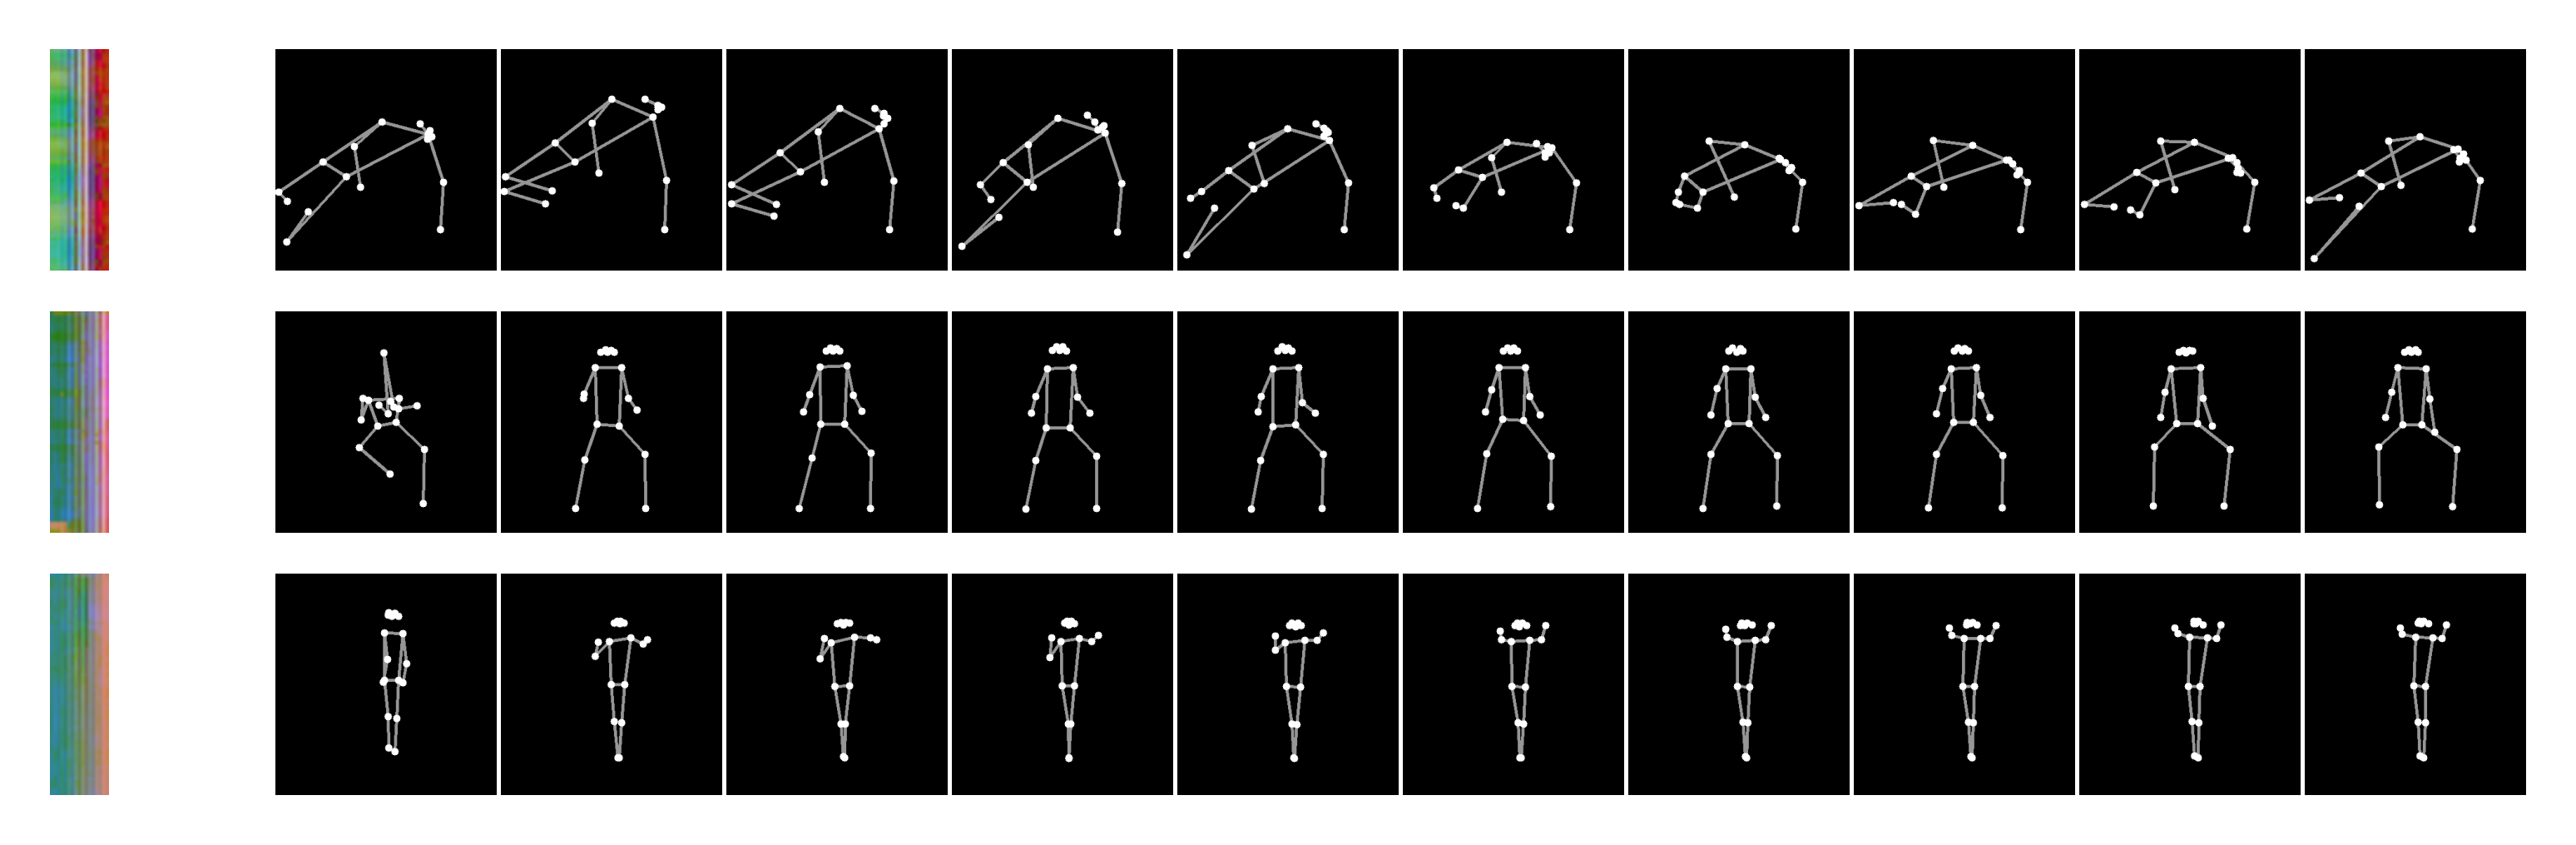
\includegraphics[width=\textwidth]{images/motion_image.png}
    \caption{Die Frames von Schlüsselpunktanimationen können als
    zweidimensionale Bilder repräsentiert werden. Die erste Reihe stellt eine
    Liegestütz-, die zweite eine Bankpress- und die dritte eine Hantelbewegung
    dar. Die erste Spalte zeigt jeweils das kodierte Bild, während die
    restlichen Spalten die ersten 10 Frames der Bewegung zeigen.}
    \label{fig:motion-images}
\end{figure}

\section{Training vom KpGAN}
Für das Training wurde der UCF-101-Datensatz \cite{ucf101} verwendet. Dieser
enthält sportliche Aktivitäten in Form von Videos, sodass diese vorerst in
Schlüsselpunktanimationen umgewandelt werden müssen. Anstatt jeden Frames jedes
Videos per Hand zu bearbeiten und Schlüsselpunkte zu annotieren, wird dies
mithilfe von MoveNet \cite{movenet} automatisiert erledigt. Die Schlüsselpunkte
der jeweiligen Frames werden in Bilder wie in Abbildung \ref{fig:motion-images}
kodiert und als Eingabe in das KpGAN gegeben. Die Experimente verlaufen ähnlich
wie beim ViGAN, es werden jedoch andere Parameter gewählt, die pro Experiment
verändert werden. Im ersten Schritt wurde untersucht, welche Netzkonfiguration
stabil beim Training ist. Das Resultat ist in Abbildung \ref{fig:kpgan} zu
sehen und wurde wie beim ViGAN durch unterschiedliche Versuche herausgefunden.
Anschließend wurde untersucht, wie sich das Verhalten während des Trainings
ändert, wenn wahlweise Batch-Normalisierung- und Bias-Layer hinzugefügt werden.
Außerdem wurde geschaut, welche Aktivierungsfunktion in der letzten Schicht zu
den besten Ergebnissen führt. Dafür wurden Aktivierungen durch Sigmoid- und
Tangens-Hyperbolicus-Funktionen realisiert. Konfigurationen mit Bias-Layer, aber
ohne Batch-Normalisierung führten zu den besten Ergebnissen. Abbildung
\ref{fig:kpgan-example} zeigt eine zufällige Liegestützbewegung, die vom KpGAN
erzeugt wurde. Für das Training stand eine RTX 3080 zur Verfügung und 3000
Epochen dauerten $< 1$ Minuten. Grundsätzlich sind die Ergebnisse
zufriedenstellend, sodass dieses GAN verwendet werden kann, um verschiedene
Bewegungen zu erzeugen.

\begin{figure}
    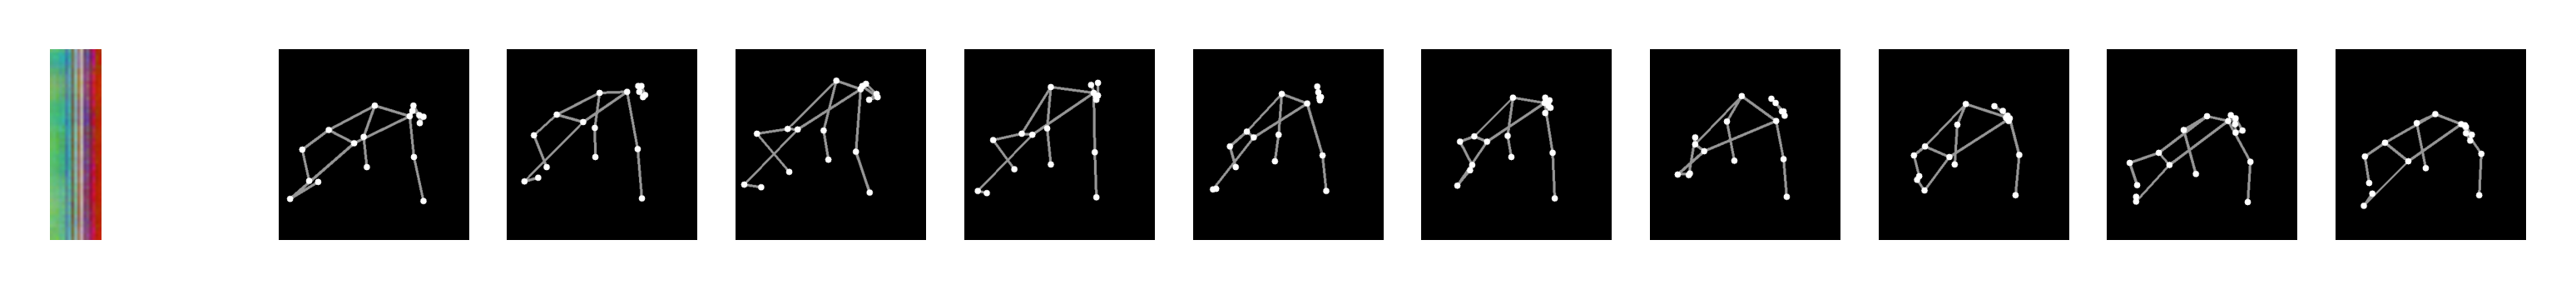
\includegraphics[width=\textwidth]{images/kpgan-example.png}
    \caption{Beispielausgabe vom KpGAN. Links ist die direkte Ausgabe des
    Netzwerks. Von links nach rechts werden chronologisch die ersten 10
    dekodierten Frames dargestellt.}
    \label{fig:kpgan-example}
\end{figure}

\begin{figure}
    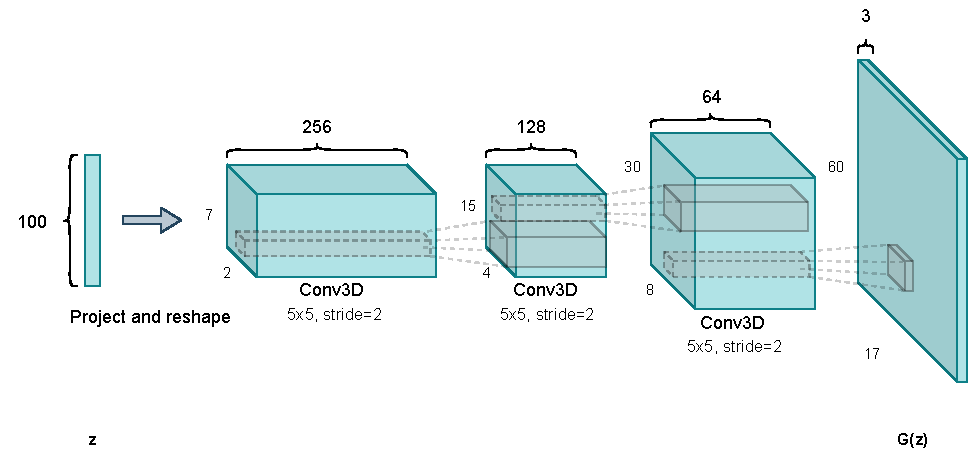
\includegraphics[width=\textwidth]{images/KpGAN.pdf}
    \caption{Architektur von KpGAN zum Generieren von Schlüs\-sel\-punkt\-anima\-tionen. Die Eingabe ist ein Vektor, welcher zunächst in das Format $7 \times 2 \times 256$ gebracht wird. Anschließend wird mithilfe von insgesamt drei Convolutional-Layer eine Ausgabe im Format $60 \times 17 \times 3$ erzeugt. Es werden entsprechend 256, 128 und 64 Filter für die Layer verwendet.}
    \label{fig:kpgan}
\end{figure}
  \chapter{Bewegungserkennung}\label{chapter:motion-detection}
In diesem Kapitel sollen die Ergebnisse aus Kapitel \ref{chapter:dataset}
verwendet werden, um eine Bewegungserkennung zu entwickeln. Genauer gesagt soll
hier ein Machine-Learning-Modell entworfen und trainiert werden, um Bewegungen zu
erkennen und klassifizieren. Zudem soll ein Ausblick auf Techniken gegeben
werden, um weitere bewegungsabhängige Eigenschaften mithilfe von KNNs zu
extrahieren. Zum Beispiel ist beim Ausüben von sportlichen Aktivitäten neben der
Bewegungsart auch interessant, ob die Bewegung richtig ausgeführt wurde. Aber
auch das Vorhersagen von zukünftigen Bewegungen anhand kürzlich getätigten Posen
kann für einige Anwendungen hilfreich sein. So auch zum Beispiel beim
vorzeitigen Erkennen von aggressiven Verhaltensmustern, sodass eingegriffen
werden kann, bevor die eigentliche Tätigkeit ausgeführt werden kann. 

Eine Bewegung kann durch die Änderung des Ortes über die Zeit beschrieben
werden. Das bedeutet, dass eine einzige Fotoaufnahme einer sich bewegenden
Person nicht ausreicht, um eine Bewegung aufzuzeichnen. Entsprechend müssen
Bilder über Zeit aufgenommen werden. Die nächste Frage, die sich ergibt ist, wie
viele Bildaufnahmen nötig sind, um eine Bewegung erkennen zu können. Dies hängt
natürlich von der Art der Bewegung und der Bewegungsgeschwindigkeit ab. Möchte
man beispielsweise einen Jumping-Jack aufnehmen und die Person bewegt sich viel
zu langsam, dann sind wesentlich mehr Aufnahmen nötig, als wenn diese sich in
einem normalen Tempo bewegen würde. In der Informationstheorie wird dies
mithilfe der Abtastrate beschrieben, die angibt, wie oft pro Sekunde abgetastet
werden soll.  Damit in Verbindung kann man die minimale Rate durch das
Niquist-Shannon-Abtasttheorem bestimmen, welches aussagt, dass ein Signal exakt
rekonstruierbar ist, wenn ein Signal mit der doppelten Abtastrate $f_{abtast} =
2 \cdot f_{max}$ abgetastet wird.

Ein durchschnittlicher Fahrradfahrer schafft eine Trittfrequenz von maximal 60
Umdrehungen pro Minute während Leistungssportler bis zu 110 Umdrehungen pro
Minute schaffen \cite{smolik}. Das würde bedeuten, dass die Abtastrate
mindestens 2 Hz betragen muss, um das Signal rekonstruierbar aufzuzeichnen.
Betrachtet man nun eine Beinpressbewegung, die ebenfalls mit 60 Tritten pro
Minute ausgeführt wird, ergibt sich ebenfalls eine Abtastfrequenz von 2 Hz. Hier
wird folgendes Problem ersichtlich. Tastet man die Fußpositionen der Sportler
mit 2 Hz ab, so kann man nicht zwischen Kreisbewegung und Linearbewegung
unterscheiden. Würde man hingegen mit 3 Hz abtasten, so wären die Bewegungen
eindeutig voneinander unterscheidbar. Dies hat unter anderem damit zu tun, dass
eine lineare Funktion durch zwei Punkte und ein Kreis stets durch drei sich
nicht auf einer Geraden befindenden Punkte beschreibbar ist. Damit also ein
neuronales Netz eine akkurate Bewegungserkennung durchführen kann, ist es
wichtig, dass dieses mit möglichst vielen Frames pro Sekunde (FPS) ausgeführt
wird, um verschiedenste Bewegungen erkennen zu können. Eine Überabtastung wird
hierbei als weniger kritisch angesehen, als eine Unterabtastung.

Für die Bewegungserkennung wird in dieser Arbeit die Erkennung von menschlichen
Posen eingesetzt, die Schlüsselpunkte des Körpers aus Bildern extrahiert. Aus
diesen Informationen können bereits einige Eigenschaften einer 
Bewegung abgeleitet oder berechnet werden. So ist zum Beispiel die Berechnung
des Winkels zwischen Oberschenkel und Wade relativ simpel, wenn die
entsprechenden Schlüsselpunkte bekannt sind. Dem Benutzer kann dadurch
berechnet werden, ob eine Übung, die abhängig von diesem Winkel ist, richtig
ausgeführt wird oder nicht. Grundsätzlich wird folgende Idee zum Erkennen bzw.
Analysieren von Bewegungen verfolgt. Die von einer Kamera
aufgenommenen Bilder werden als Eingabe in einen Pose-Detektor gegeben, welcher
zunächst die in dem Eingabebild enthaltenen Schlüsselpunkte ausgibt.  Diese
werden dann anschließend in einen angehängten Prediction-Head gegeben, welcher
dann aus den Schlüsselpunkten die Bewegungsart erkennt.

\section{Erkennung von menschlichen Posen}
Das Erkennen von menschlichen Posen hat in den letzten Jahren viel
Aufmerksamkeit bekommen und wird in 2D- bzw. 3D-Human-Pose-Estimation (HPE)
unterschieden. Diese Arbeit beschäftigt sich mit der 2D-HPE, um Schlüsselpunkte
des menschlichen Körpers in Bildern zu detektieren. Auch wird sich auf die
Erkennung von Einzelpersonen in Bildern konzentriert, anstatt viele
verschiedene Personen gleichzeitig zu bestimmen. Hierbei spricht man von
Single-Person-Pipelines, die wiederum in zwei unterschiedliche Methoden
unterteilt werden: Regressions- und Körperteildetektionsmethoden
\cite{zheng2021deep}.

Mit Regressionsmethoden werden zu Eingabebildern direkt die Schlüsselpunkte
ausgegeben. Dabei soll ein KNN lernen, Bilder auf Schlüsselpunktkoordinaten
abzubilden. Die Ausgabe besitzt dementsprechend $k \cdot n$ Komponenten, wobei
$k$ die Anzahl der Schlüsselpunkte und $n$ die Anzahl der Eigenschaften pro
Schlüsselpunkt angibt. Das Problem bei dieser Methode ist, dass Körperteile wie
Hände, Augen und Füße in einem Bild sehr klein ausfallen können. Dort ist es
dann sehr schwer, diese von der Umgebung unterscheiden zu können und damit eine
präzise Aussage darüber zu treffen, wo sich deren Schlüsselpunkte befinden.
Auch ist es möglich, dass einige Körperteile nicht auf dem Bild zu sehen sind.
Das Treffen einer Aussage, ob das entsprechende Körperteil überhaupt im Bild
vorhanden ist, gestaltet sich bei dieser Methode eher schwierig. Hierbei kann
die folgende Methode helfen.

Bei Körperteildetektionsmethoden verläuft die Erkennung von Schlüsselpunkten ein
wenig anders. Anstatt direkt auf Koordinaten der Schlüsselpunkte abzubilden,
versucht man hier eine Reihe von Wärmekarten zu erzeugen. Genauer ausgedrückt
wird für $k$ Schlüsselpunkte eine Menge aus Wärmekarten $H = \{H_1, ..., H_k\}$
erzeugt. Eine Wärmekarte $H_i$ enthält dabei für jedes Koordinatenpaar $(x, y)$
einen Wahrscheinlichkeitswert $p_{y, x} \in H_i$, welcher angibt, zu welcher
Wahrscheinlichkeit dort ein Schlüsselpunkt vorliegt.  Für das Training solcher
Modelle wird meistens die Abweichung zwischen generierten und tatsächlichen
Wärmekarten mit Hilfe des Mean-Squared-Errors (MSE) minimiert. Grund\-sätz\-lich
besitzen Körperteildetektionsmethoden den Vorteil, dass auch relativ kleine
Körperteile gut erkannt werden. Der Unterschied zwischen den Methoden ist in
Abbildung \ref{fig:pose-detection} zu sehen. Es werden in aktuellen Forschungen
bezüglich der Posenerkennung häufig Modelle, die Wärmekarten erzeugen, verwendet
\cite{zheng2021deep}.

\begin{figure}
    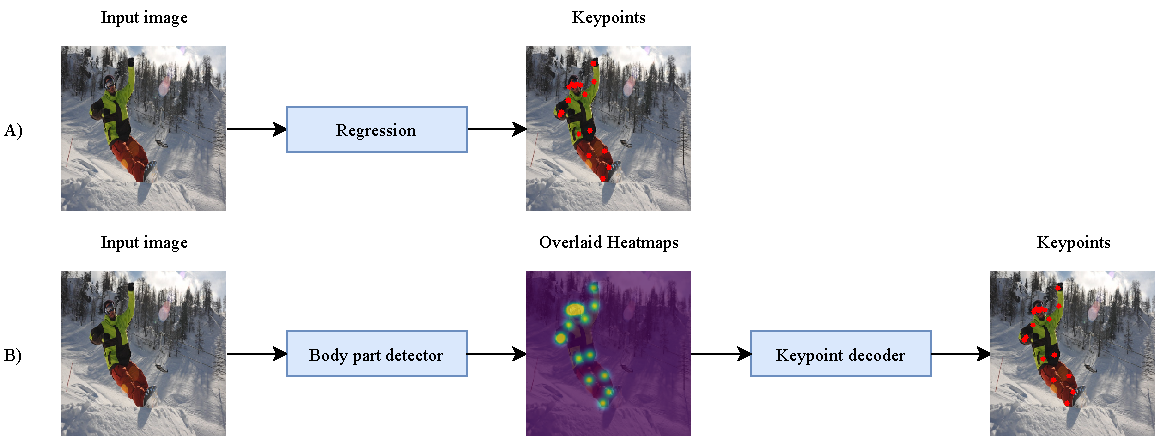
\includegraphics[width=\textwidth]{images/pose_detection.pdf}
    \caption{Regressions- und Körperteildetektions-Verfahren
    zum Be\-stim\-men von Schlüs\-sel\-punk\-ten eines Menschen. A) Ein Regressor
    versucht direkt die Punkte des menschlichen Körpers als Koordinaten
    auszugeben. B) Ein Körper\-teil\-detektor erzeugt eine Wärmekarte für jeden
    Schlüsselpunkt. Die Werte in den Karten geben die Wahrscheinlichkeit für den
    Aufenthalt eines Punktes an. Die Schlüsselpunkte müssen nach der Detektion aus den Karten dekodiert werden.}
    \label{fig:pose-detection}
\end{figure}

Ein Forschungsteam von Google hat ein neues Machine-Learning-Modell namens
\textit{MoveNet} \cite{movenet} präsentiert, das unter anderem auf mobilen
Geräten ausgeführt werden kann und dabei eine Echtzeiterkennung von menschlichen
Posen ermöglicht. Die Architektur besteht aus einem MobileNetV2-Backbone mit
angehängtem Feature-Pyramid-Network (FPN) und insgesamt vier Prediction-Heads,
die CenterNets \cite{zhou2019objects} sind. Trainiert wurde das Netzwerk
auf den COCO-Datensatz und erreicht laut den Autoren 30 oder mehr FPS auf
modernen Computern, Laptops und Smartphones. Auch dieses Modell verwendet
Wärmekarten, um mögliche Positionen von menschlichen Schlüsselpunkten zu
bestimmen und wird von einem Prediction-Head übernommen. Ein weiterer ist dafür
zuständig, den Abstand (Offset) jedes Pixels als Vektor von der geschätzten
Schlüsselpunktposition zu bestimmen. Ein anderer Kopf übernimmt die Gruppierung
der Schlüsselpunkte und ordnet diesen Personeninstanzen zu. Der vierte Kopf
schätzt das Zentrum der Instanzen. Die vollständige Architektur von MoveNet ist
in Abbildung \ref{fig:movenet-architecture} zu sehen. MoveNet verwendet also
neben dem Erzeugen von Körperteildetektionsmethoden zum Erzeugen von Wärmekarten
auch Regressionsmethoden, um die Position von Schlüsselpunkten noch genauer
angeben zu können.

\begin{figure}
    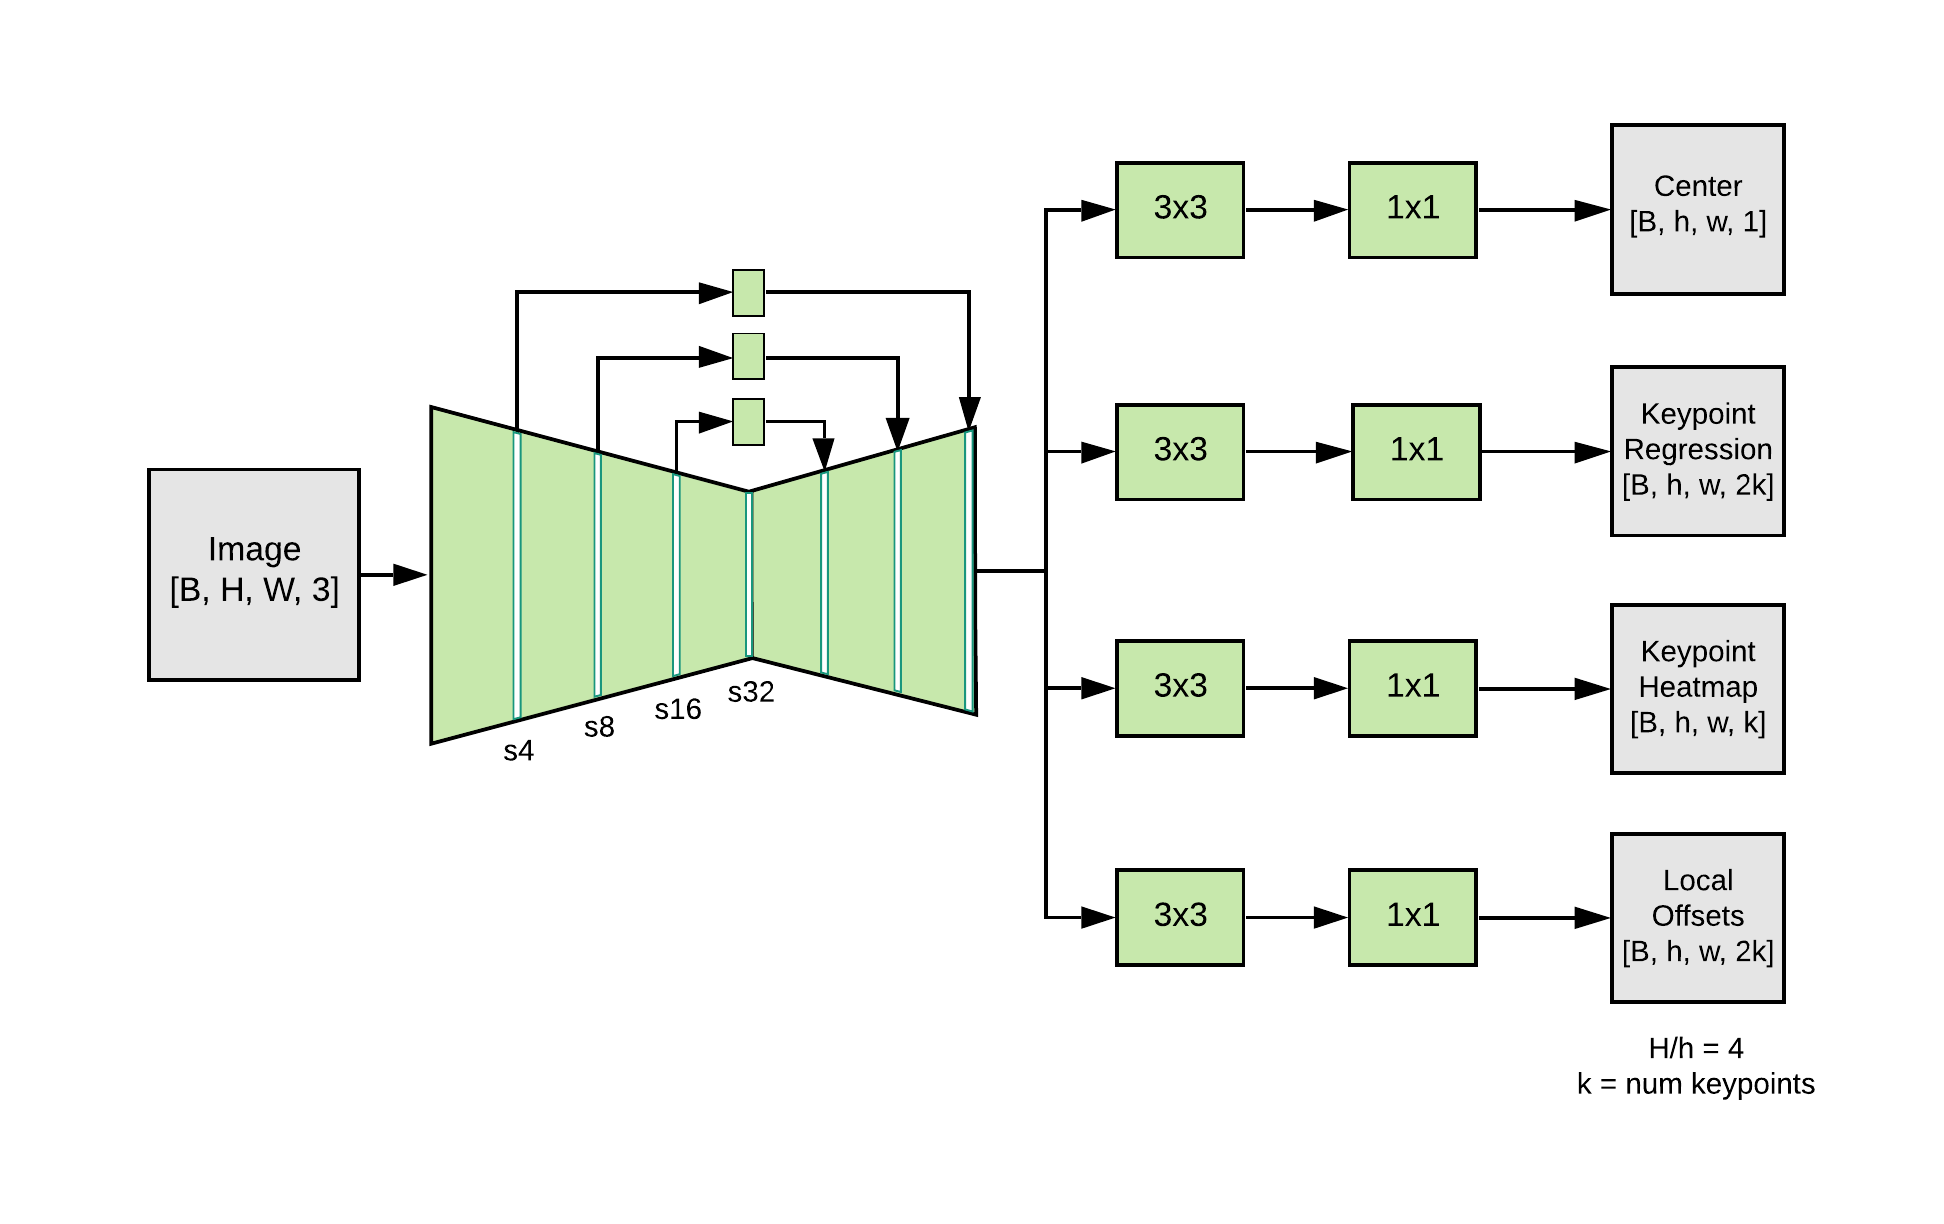
\includegraphics[width=\textwidth]{images/movenet_architecture.png}
    \caption{Architektur von MoveNet \cite{movenet}. Der Feature-Extractor
    besteht aus einem vortrainierten MobileNetV2-Backbone mit angehängtem FPN.
    Insgesamt werden vier Prediction-Heads zum Bestimmen von Schlüsselpunkten
    verwendet.}
    \label{fig:movenet-architecture}
\end{figure}

\section{Erkennung von Bewegungsarten}
Bei der Erkennung von Bewegungsarten handelt es sich um ein
Klassifizierungsproblem, bei der es darum geht, einer Bewegungsaufzeichnung
eine Klasse zuzuweisen. Zu einer beliebigen Bewegungssequenz soll also eine
Aussage getroffen werden, ob es zum Beispiel Hantelübungen sind. Im Laufe dieses
Abschnitts soll dementsprechend ein Machine-Learning-Modell namens MotionNet
entworfen werden, welches auf diese Aufgabe trainiert wird. Hierzu muss vorerst
definiert werden, welche Daten verwendet werden und wie diese für das Training
vorbereitet werden können. Damit eine Ortsänderung eines zu betrachtenden
Objektes aufgezeichnet werden kann, müssen mehrere Bilder bzw. Videos
aufgezeichnet werden. Eine Bewegung anhand eines einzelnen Bildes ist nicht
möglich, da die Information über die Ortsänderung dann nicht vorhanden ist. Es
gilt also einen Datensatz zu finden, welcher verschiedene Bewegungen im
Videoformat bereitstellt. Alternativ muss ein entsprechender Datensatz
ausgehoben werden, was einen relativ hohen Zeitaufwand bedeuten würde. Es wird
aufgrund seiner Einfachheit der UCF-101-Datensatz \cite{ucf101} verwendet.
Dieser besteht aus 101 Bewegungsarten in Form von Videos, die öffentlich auf der
Plattform YouTube zur Verfügung stehen. Ein Videoclip ist dabei eindeutig einer
Bewegungsklasse zugeordnet. Um den Datensatz künstlich zu erweitern bzw. um eine
Augmentation durchzuführen, wird das KpGAN aus Kapitel \ref{chapter:gans}
verwendet. Dieses erzeugt während des Trainings Schlüsselpunktdaten auf
Nachfrage. Zur Unterscheidung wird im Folgenden der UCF-101-Datensatz als realer
Datensatz bezeichnet.

Es wird nun ein Modell entworfen, welches $n$ Frames eines Videos einliest und
die geschätzte Bewegungsklasse für diese Frames ausgibt. Dabei soll das Netzwerk
lernen, menschliche Posen aus den Frames zu extrahieren und anschließend zu
klassifizieren. Da das Neutrainieren der Posenerkennung zu lange dauern würde,
wird ein vortrainiertes MoveNet als Backbone verwendet. Für die Klassifizierung
werden verschiedene Köpfe implementiert, die anschließend miteinander verglichen
werden. Ziel ist es herauszufinden, welche Architekturen für den Gebrauch auf
mobilen Plattformen geeignet sind.

Die zu betrachtenen Metriken sind Genauigkeit und
Aus\-führ\-ungs\-ge\-schwin\-dig\-keit. Als erstes werden einfache
Fully-Connected-Layer verwendet und evaluiert. Es wurden dabei Schritt für
Schritt Änderungen an der Anzahl der Neuronen und Schichten vorgenommen.
Anschließend wird untersucht, ob das Verwenden CNNs ähnliche oder bessere
Ergebnisse liefert, besonders in Hinblick auf die Performance. In Tabelle
\ref{table:motion-detection} sind die durchgeführten Experimente aufgelistet.

Das Ergebnis aus den Trainingsversuchen mit rein-realen Datensätzen ist, dass
CNNs die Bewegungen wesentlich besser erkennen können als die
Fully-Connected-Modelle. Nicht nur, dass sie hier eine höhere Genauigkeit
aufweisen, sie lernen die Verteilung auch wesentlich schneller. Während die
Fully-Connected-Modelle 300 Epochen für eine Genauigkeit von 90-97\% benötigen,
benötigen die CNNs lediglich 9-80 Epochen für bessere Resultate. Der einzige
Nachteil besteht in ihrer Ausführungsgeschwindigkeit, die bis zu vier mal
kleiner ist.

Erstaunlicherweise verhält sich dies bei den Trainingsversuchen mithilfe eines
GANs ein wenig anders. Grundsätzlich erreichten die Fully-Connected-Modelle eine
wesentlich höhere Genauigkeit nach sehr viel weniger Trainingsepochen. Die
Genauigkeit wurde dabei nicht mithilfe von synthetischen Daten des GANs
gemessen, sondern es wurden hierfür wieder echte Daten verwendet. Damit wurde
sichergestellt, dass die Genauigkeiten der verschiedenen Trainingsmethoden
vergleichbar gehalten werden. Das Verwenden von künstlich erzeugten Daten
liefert in diesem Fall also immer bessere Ergebnisse. Dies liegt vermutlich
unter anderem daran, dass GANs die Eigenschaft besitzen, zwischen echten Daten
zu interpolieren und damit automatisch eine Augmentation durchzuführen. Dies
führt dazu, dass die Modelle eine höhere Vielfalt lernen können. Diese Vielfalt
ist im echten Datensatz nicht so ausgeprägt. Hierbei ist wichtig zu erwähnen,
dass das Daten erzeugende GAN auf eben diesen Datensatz trainiert wurde. Der
Datensatz wurde also verbessert, indem ein GAN verwendet wurde, die Verteilung
zu lernen und zu interpolieren, um eine größere Datenvielfalt zu erzeugen.

Für den Rest dieser Arbeit wird MotionNet als CNN verwendet, die hier die besten Ergebnisse erzielt wurden.

\begin{table}
    \footnotesize
    \begin{tabularx}{\textwidth}{l|X||c|c||c|c||c}
        \hline
        Network Type & Layers & $e_\mathrm{real}$ & $p_\mathrm{real}$ & $e_\mathrm{gan}$ & $p_\mathrm{gan}$ & Inference Speed (s) \\ \hline

        \multirow{3}{*}{linear} & Dense, 128 \newline ReLU \newline Dense, 3 & 300 & 0.90 & 82 & 0.99 & \num{0.59e-6} \\ \cline{2-7}

        & Dense, 256 \newline ReLU \newline Dense, 3 & 300 & 0.94 & 49 & 0.99 & \num{0.61e-6} \\ \cline{2-7}

        & Dense, 128 \newline ReLU \newline Dense, 256 \newline ReLU \newline Dense, 3 & 300 & 0.97 & 70 & 0.99 & \num{0.83e-6} \\ \hline

        \multirow{3}{*}{conv} & Conv2D, 16, $3 \plh 3$, stride 2 \newline Conv2D, 32, $3 \plh 3$, stride 2 \newline Dense, 3 & 81 & 0.99 & 123 & 0.99 & \num{1.25e-6} \\ \cline{2-7}

        & Conv2D, 16, $3 \plh 3$, stride 2 \newline Conv2D, 32, $3 \plh 3$, stride 2 \newline Conv2D, 64, $3 \plh 3$, stride 2 \newline Dense, 3 & 44 & 0.99 & 121 & 0.99 & \num{1.74e-6} \\ \cline{2-7}

        & Conv2D, 16, $3 \plh 3$, stride 2 \newline Conv2D, 32, $3 \plh 3$, stride 2 \newline Conv2D, 64, $3 \plh 3$, stride 2 \newline Conv2D, 128, $3 \plh 3$, stride 2 \newline Dense, 3 & 9 & 0.99 & 126 & 0.99 & \num{2.27e-6} \\ \hline
    \end{tabularx}
    \caption{Durgeführte Experimente mit verschiedenen Architekturen für die
    Bewegungserkennung. Die Eingabe besteht aus 60 Frames einer
    Bewegungsanimation aus 17 Schlüsselpunkten mit jeweils 3 Eigenschaften (x-,
    y-Koordinaten und Wahrscheinlichkeitsscore) kodiert als Bild (siehe
    Abbildung \ref{fig:motion-images}). Als Ausgabe sollen die Netze die
    geschätzte Klasse, also das Label liefern. $p_\mathrm{real}$ gibt die
    Genauigkeit des jeweiligen Modells an, das mit einem realen Datensatz
    trainiert wurde. $p_\mathrm{gan}$ gibt hingegen die Genauigkeit der Modelle
    an, die mithilfe eines KpGAN-Generators trainiert wurden. $e_\mathrm{real}$ und $e_\mathrm{gan}$ sind entsprechende Trainingsepochen. Für das Messen der
    Genauigkeit wurden immer reale Daten verwendet.}
    \label{table:motion-detection}
\end{table}

  \include{sections/discussion.tex}
  \chapter{Fazit und Ausblick}
In dieser Thesis wurden verschiedene Modelle des maschinellen Lernens entwickelt
und evaluiert. Vor allem wurden sogenannte Generative-Adversarial-Networks
(GANs) erforscht und neue Methoden zum Erzeugen von künstlichen Bewegungen
gesucht, um einen kompletten Datensatz mithilfe eines solchen Modells zu
erzeugen. Als Ergebnis wurde zuerst ViGAN präsentiert. Ziel von ViGAN ist es,
aus einem bestehenden Video-Datensatz neue bisher unbekannte Proben zu erzeugen.
Dies gelang auch bis zu einem gewissen Grad. Es wurden zwar neue Videos vom
Netzwerk erzeugt, jedoch konnte nicht sichergestellt werden, ob sich eine Person
tatsächlich bewegt oder still steht.  So sind Personen oft regungslose starre
Körper, während sich z.B. ganze Räume über die Zeit verändern. Als Alternative
dazu wurde KpGAN entworfen, welches direkt verschiedenste Bewegungsanimationen
erzeugen kann. Diese Bewegungsanimationen bestehen dabei aus menschlichen
Schlüsselpunkten und werden als Bilder kodiert.  Experimente haben gezeigt, dass
Datensätze, die komplett mithilfe von KpGAN erzeugt wurden, mindestens genau so
gut für das Training anderer Modelle geeignet sind, wie entsprechende reale
Datensätze.  Dies bringt einen großen Vorteil mit sich, denn der eigentliche
Datensatz kann ohne großen Aufwand beliebig erweitert werden, während beim
realen Datensatz ein signifikanter Zeitaufwand entstehen würde.

Im Anschluss wurden mithilfe von KpGAN weitere neuronale Netzwerke trainiert,
die Bewegungen aus Schlüsselpunktsequenzen erkennen sollen.  Die Herausforderung
ist dabei die Echtzeiterkennung auf mobilen Geräten. Die verwendeten Metriken
waren Genauigkeit und Performance. Aus den Experimenten resultierte schließlich
das MotionNet, welches eine sehr gute Erkennungsrate und Ausführungsgeschwindigkeit
besitzt.  Mithilfe des trainierten MotionNets und eines externen Modells von
Google (MoveNet-Lightning) wurde anschließend eine mobile App entwickelt, welche
die Anwendbarkeit und Performance auf mobilen Geräten messen soll. Auf modernen
Smartphones wurde eine Aus\-führ\-ungs\-ge\-schwindig\-keit von bis zu 14 FPS
gemessen. Auch wurde durch Praxistests bewiesen, dass eine Bewegungserkennung
auf modernen und älteren mobilen Plattformen in Echtzeit ausführbar ist und
tatsächlich Bewegungen erkennt. Damit wurde die Forschungsfrage, ob eine
Bewegungserkennung auf mobilen Geräten in Echtzeit ausgeführt werden kann,
beantwortet und eine Beispiel-App präsentiert.

Weiterführende Arbeiten können sich in Zukunft mit dem Verbessern des ViGAN
be\-schäf\-tigen, um das Problem mit den sich nicht bewegenden Personen in
Videos zu lösen. Zudem kann das MotionNet um weitere Bewegungen erweitert
werden. Die hier vorgestellte Lösung zum Erkennen von Bewegungen findet
lediglich im zweidimensionalen Raum statt. Interessant wäre es zu wissen, ob
eine dreidimensionale Repräsentation der menschlichen Schlüsselpunkte zu anderen
Ergebnissen führen würde. Dies könnte in Zukunft ebenfalls weiter
untersucht werden.


  \printbibliography
\end{document}
